\documentclass[a4paper,11pt]{book}


\usepackage[top=2cm,bottom=2cm,left=2cm,right=2cm]{geometry}
\usepackage[pdftex]{graphicx} %per poter inserire le figure
\usepackage{amssymb,amsmath,amsthm,amsfonts}
\usepackage{xspace}
\usepackage{tabularx}
\usepackage{indentfirst}
\usepackage{subfigure}
\usepackage[small]{caption}
\usepackage{eucal}
\usepackage{eso-pic}
\usepackage{url}
\usepackage{booktabs}
\usepackage{afterpage}
\usepackage{parskip}
\usepackage{listings}
\usepackage{fancyhdr}
\usepackage{textcomp}
\usepackage{cite}
\usepackage{multirow}
\usepackage[utf8]{inputenc}   %per riuscire a scrivere gli accenti
\usepackage[italian]{babel}    %per riuscire a scrivere gli accenti
\usepackage{setspace}
\usepackage{graphicx,wrapfig,lipsum}
\usepackage{bm}
\pagestyle{fancy}




\begin{document}

\begin{titlepage}
\vspace{5mm}
\begin{figure}[hbtp]
\centering

\includegraphics[scale=.13]{logo_unipd.png}
\end{figure}
\vspace{5mm}
\begin{center}
{{\huge{\textsc{\bf UNIVERSIT\`A DEGLI STUDI DI PADOVA}}}\\}
\vspace{5mm}
{\Large{\bf Dipartimento di Fisica e Astronomia ``Galileo Galilei''}} \\
\vspace{5mm}
{\Large{\textsc{\bf Corso di Laurea in Fisica}}}\\
\vspace{20mm}
{\Large{\textsc{\bf Tesi di Laurea}}}\\
\vspace{30mm}
\begin{spacing}{3}
{\LARGE \textbf{Track reconstruction of trigger-less drift tubes chambers}}\\
\end{spacing}
\vspace{8mm}
\end{center}

\vspace{20mm}
\begin{spacing}{2}
\begin{tabular}{ l  c  c c c  cc c c c c  l }
{\Large{\bf Relatore}} &&&&&&&&&&& {\Large{\bf Laureando}}\\
{\Large{\bf Prof. Marco Zanetti}} &&&&&&&&&&& {\Large{\bf Mattia Pujatti}}\\
\end{tabular}
\end{spacing}
\vspace{15 mm}

\begin{center}
{\Large{\bf Anno Accademico 2018/2019}}
\end{center}
\end{titlepage}


\clearpage{\pagestyle{empty}\cleardoublepage}

\tableofcontents


\chapter*{Abstract}

A re-scaled and revisited version of the CMS drift tubes muon chambers has been designed to be used at beam tests and for
tomography applications. A set of chambers of this type have been produced at the INFN Legnaro Laboratory in 2018 and 2019. An
important feature of those detectors is their handiness, i.e. they can be arranged to best fit the experimental needs. It is therefore
important to develop a reconstruction algorithm flexible enough to address multiple geometrical configurations; at the same time,
dedicated suites have to be deployed to allow a fast determination of alignment and calibration constants. Furthermore, the readout
of those detectors do not require a trigger signal, i.e. (zero-suppressed) data are continuously sampled from the front-ends. In view
of an online analysis running on the unfiltered data, the track reconstruction must be fast, little sensitive to noise and developed with
software tools that can best fit in an online environment. The thesis work will focus on the development of algorithms which satisfy
the requirements listed above.




\part{The Physics behind the muon detectors}


\chapter{Track Detectors}
\section{Gaseous Ionization Detectors}
Le camere a drift fanno parte dei cosìdetti rivelatori gassosi di ionizzazione, che sfruttano il passaggio della radiazione ionizzante attraverso un gas per produrre, ad ogni interazione, delle coppie elettrone-ione positivo. Ai capi di tali dispositivi sono presenti due elettrodi, tra i quali viene stabilita un'opportuna differenza di potenziale, che permette di stabilire un campo elettrico uniforme e costante all'interno della camera. Le cariche di ionizzazione prodotte vengono attirate verso le estremità della macchina (gli elettroni verso l'anodo e gli ioni positivi verso il catodo) e raccolte da un circuito che genera un segnale che verrà in seguito analizzato.\\
La differente mobilità degli elettroni rispetto agli ioni, fa sì che i primi arrivino a destinazione molto in anticipo, e perciò è spesso conveniente limitarsi a raccogliere solo quel tipo di cariche, che comunque generano un segnale sufficiente che, nel peggiore dei casi, può essere amplificato prima dell'analisi.\\
I gas più utilizzati all'interno di questi rivelatori sono Boro, Elio e Argon, ma comunque sempre sostanze allo stato gassoso, perchè, sebbene liquidi e solidi aumentino il numero di interazioni possibili grazie alla loro maggiore densità, allo stesso tempo possono limitare la mobilità della carica ionizzante all'interno della camera, causando ritardi nella raccolta e segnali più rumorosi. Il vantaggio apportato da questi gas nobili è riconducibile alla completezza delle loro shell elettroniche, cosa che fa sì che l'energia delle particelle venga dissipata quasi interamente per la ionizzazione. Inoltre, la mancanza di elettronegatività previene la cattura di elettroni e la dannosa creazione di ioni negativi.\\

Di seguito, in figura \ref{fig:gas_ion_ch_scheme}, viene riportato lo schema di funzionamento di un rivelatore di ionizzazione:

\begin{figure}[hbtp]
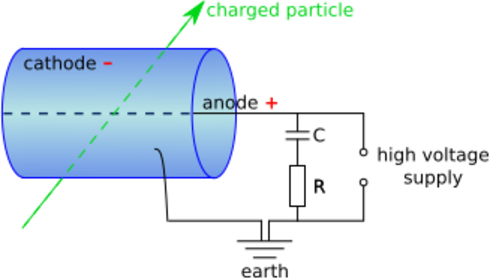
\includegraphics{pictures/gas_ion_det.pdf}
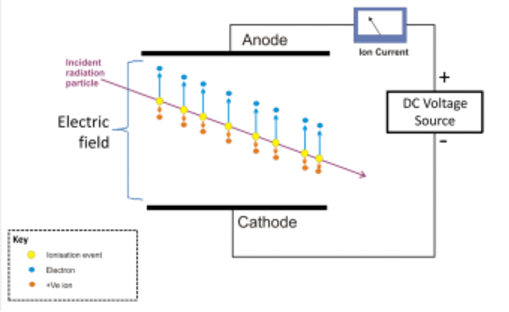
\includegraphics{pictures/gas_ion_det_2.pdf}
\caption{Scheme for a gaseous ionization chamber}
\label{fig:gas_ion_ch_scheme}
\end{figure}

Gli elettroni di ionizzazione raggiungono quindi l'anodo e, accumulandosi sulle armature della capacità C, aumentano la tensione sulla resistenza e danno origine ad un segnale impulsivo (pulse) attraverso di essa, che viene registrato elettronicamente.\\

Come è noto, la variazione di potenziale sul condensatore, e quindi indirettamente quella sulla resistenza, è direttamente proporzionale alla variazione della carica accumulata sulle armature ($\Delta Q = \Delta V/C$), che è proprio pari al numero di elettroni raccolti nell'anodo. Ma la quantità di cariche raccolta nell'anodo dipenderà dal numero effettivo di interazioni avvenute tra le molecole del gas presente nella camera e la particella ionizzante, numero al quale bisogna però moltiplicare un opportuno fattore di amplificazione (che si può chiamare \textit{A}) che tiene conto di una possibile seconda ionizzazione. Se i prodotti della prima ionizzazione sono infatti sufficientemente energetici, non è da escludere che il fenomeno possa ripetersi.\\
Detto \textit{n$\cdot$e} il numero di cariche che prodotte dalla prima ionizzazione, l'altezza del segnale raccolto dall'elettronica è:\\
\[ \text{Pulse height = } \Delta V = A\frac{n\cdot e}{C} \]

Si osserva, per questo genere di detector, che la carica di ionizzazione dipende in maniera importante dall'intensità del campo elettrico stabilito all'interno dell'apparato, tanto da definire diverse regioni di lavoro, rappresentate dal grafico \ref{fig:ion_ch_work_regions}.\\


\begin{figure}[hbtp]
\centering
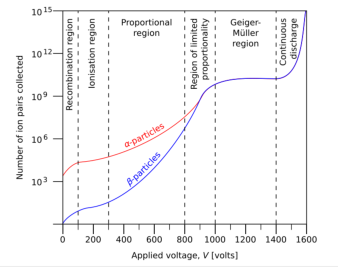
\includegraphics[scale=1.5]{pictures/work_region_det.pdf}
\caption{Ionization charge vs electric field intensity in a gaseous ionization chamber}
\label{fig:ion_ch_work_regions}
\end{figure}

% Descrivere tutte le regioni di lavoro dei rivelatori?

La più importate tra di queste, quella su cui operano la maggior parte dei rivelatori di radiazione, è la \textit{regione proporzionale}, caratterizzata da un forte gradiente di potenziale in prossimità dell'anodo, il quale permette la formazione di un fenomeno noto come \textit{valanga Townsend}. La presenza di un sufficientemente intenso campo elettrico permette agli elettroni di ionizzazione di accelerare e, urtando tra di loro o con le molecole del gas, di acquisire sufficiente energia da produrre un'ulteriore ionizzazione e una conseguente "valanga" di nuove cariche.\\
Il vantaggio di avere una valanga è che la carica viene moltiplicata per un fattore molto grande (tipicamente intorno a $10^4$ / $10^6$) e quindi il segnale che si induce sull'anodo è molto intenso, e sopratutto \textit{proporzionale} alla carica rilasciata durante la prima ionizzazione.\\



\subsection{Proportional Counters}
I detector che lavorano della regione proporzionale sono i più utilizzati: il campo elettrico all'interno è moderatamente elevato, cosa che permette una completa ma controllata amplificazione del segnale, rendendolo quindi più leggibile, senza perdere la relazione di proporzionalità con la carica di ionizzazione rilasciata nel dispositivo (cosa che può succedere con campi eccessivamente forti).\\
Le costanti di proporzionalità sono inoltre sufficientemente alte ($\sim 10^4$) da permettere l'osservazione anche di particelle di energia medio bassa ($<10\text{ keV}$).\\
La tensione risulta essere abbastanza elevata da permettere la raccolta completa delle cariche nel giro di pochi microsecondi, e quindi da costruire un segnale impulsivo registrato dall'elettronica, che può essere utilizzato per ricavare una stima dell'energia della particella. Tutto questo comunque funziona perchè la geometria dei detector consente al campo elettrico di accelerare gli elettroni solo quando questi si trovano a pochi micrometri dall'anodo: in tal modo ogni elettrone genera la stessa valanga, indipendentemente dalla posizione in cui è stato prodotto o da quanto spazio ha percorso prima di giungere all'elettrodo.\\ 
Sfortunatamente, c'è un effetto secondario da considerare: per ogni elettrone di ionizzazione c'è uno ione positivo di gas che, con una certa probabilità, può riassorbire tale elettrone, emettendo un fotone. Questo fotone può poi andare incontro ad effetto fotoelettrico e produrre un nuovo elettrone, che viene raccolto provocando la formazione di una parte "spuria" di segnale. Talvolta possono formarsi vere e proprie correnti, talmente intense dall'andare a rovinare i cavi del circuito. Per questo motivo solitamente il gas utilizzato è composto di una miscela al 10\% di un gas "estintore", tipicamente diossido di carbonio o metano, che si preoccupa di assorbire eventuali fotoni prodotti all'interno della camera, dissipando l'energia così raccolta in forme diverse (collisioni elastiche e dissociazioni) in modo da smorzare il processo secondario e prevenire l'instaurarsi di dannosi regimi di scarica.\\


\section{Multi-Wire Proportional Chambers}

Una 	\textit{multiwire proportional chamber} (MWPC) è sostanzialmente una disposizione planare di \textit{proportional counters}, equidistanti, solitamente a pochi millimetri l'uno dall'altro, posizionati in mezzo a due piastre.  I cavi dei singoli contatori fungono da anodi, mentre le due piastre da catodi, generando un campo elettrico abbastanza uniforme all'interno della camera, distorto (e più intenso) solo in prossimità di questi cavi ($E \sim 1/r$), come si evince nella figura \ref{fig:multiwire_scheme}, a sinistra.\\
La particolarità di queste multiwire chambers risiede nel fatto che ogni contatore agisce in maniera indipendente: al passaggio di radiazione ionizzante, infatti, solo il cavo più vicino raccoglie la carica prodotta generando il segnale. Questo permette di avere quindi anche un'informazione spaziale sul passaggio della particella carica, e consente di ricostruirne la traccia disponendo, ad esempio, una seconda camera a $90^\circ$ rispetto alla prima, in quanto una forte limitazione risiede nel fatto che la singola camera permette di ricavare soltanto la coordinata perpendicolare al cavo, e non quella lungo di esso.\\

\begin{figure}[hbtp]
\centering
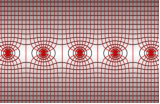
\includegraphics[scale = 2]{pictures/MWPC_electric_field.pdf} \qquad\qquad
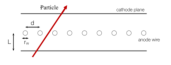
\includegraphics[scale=3]{pictures/multiwire.pdf}
\caption{Scheme for a multiwire chamber}
\label{fig:multiwire_scheme}
\end{figure}

Per quanto riguarda la risoluzione spaziale delle camere, ovvero la precisione sperimentale sulla traccia lasciata dalla particella che le ha attraversate, si ha che questa è inversamente proporzionale alla distanza fra i singoli cavi: più vicini sono tra loro gli anodi, maggiore è la precisione sulla posizione esatta di passaggio della radiazione. Dal punto di vista dell'analisi statistica, l'errore su un'eventuale misura di posizione si può ottenere in prima approssimazione applicando una distribuzione uniforme tra un cavo e quello adiacente ($\sigma_x = d/\sqrt{12})$), ottenendo circa 300 $\mu m$ per degli anodi disposti ad 1 mm di distanza l'uno dall'altro.\\
 A causa della repulsione elettrostatica, comunque, è presente un limite inferiore alla distanza alla quale i cavi possono essere posizionati, cosa che limita notevolmente la precisione dell'apparato, grazie al quale si raggiungono risoluzioni tipiche abbastanza basse, dell'ordine delle centinaia di $\mu m$.\\


\section{Drift Chambers}
La limitata risoluzione associata alle multiwire chambers può essere fortemente migliorata se si va a considerare il tempo di drift degli elettroni di ionizzazione: andando a misurare il lasso temporale che intercorre tra la produzione di questi e il loro raccoglimento nell'anodo, e conoscendo la velocità di deriva di tali cariche $v_d$ all'interno del gas, si può giungere ad una stima ancora più precisa della posizione in cui la radiazione ionizzante è passata, semplicemente sfruttando la relazione \ref{eq:drift_space}.
\begin{equation}
\label{eq:drift_space}
x = \int^{t_d}_{t_0} v_d dt
\end{equation}
Nel caso in cui la velocità di deriva sia costante, l'espressione diventa lineare e più semplice: $x = v_d\cdot t$.\\
Altri tipi di detector, più veloci, come gli scintillatori, sono usati per segnalare l'istante di arrivo della particella all'entrata della camera.\\

\begin{figure}[hbtp]
\centering
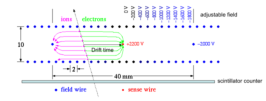
\includegraphics[scale=2]{pictures/drift_chamber_scheme.pdf}
\caption{Scheme of a drift chamber}
\label{fig:drift_chamber_scheme}
\end{figure}

La possibilità di sfruttare questi tempi di deriva consente di ridurre notevolmente il numero di cavi da utilizzare, rispetto alle multiwire, oppure di aumentare ulteriormente la risoluzione spaziale, scegliendo spaziature tra i fili sempre più piccole. Considerando infatti un tipico valore per la velocità di drift, $v_d = 5 cm/\mu s$, e un'errore casuale sul tempo dell'elettronica di $\sigma_t = 1ns$, si ottiene una risoluzione spaziale di circa $\sigma_x = v_d\cdot \sigma_t = 50 \mu m$, cioè molto più piccola che nel caso delle multiwire. Questo comporta però anche un aspetto negativo: le camere a deriva sfruttano lunghezze di drift mediamente maggiori degli altri dispositivi, e pertanto sono inevitabilmente più lente, cosa che le rende meno adatte ad essere utilizzate nei collider (troppe tracce in troppo poco tempo) o come sistemi di trigger.\\
Nel caso di camere planari, quelle in cui la deriva degli elettroni avviene sullo stesso piano in cui sono posti i fili, è necessario assicurarsi che le velocità delle cariche siano abbastanza costanti, così da semplificare i conti successivi, e pertanto occorre tenere sotto controllo il campo elettrico interno, per far sì che rimanga uniforme e costante nel tempo. Tuttavia, come noto, le linee di campo, in prossimità degli anodi, risultano molto più fitte e distorte, cosa che viene bilanciata introducendo, in mezzo a questi anode-wires, dei potential-wires, che fungono da nuovi catodi e "correggono" la non uniformità del campo.\\ 

Sono essenzialmente quattro gli effetti spuri che limitano la risoluzione spaziale delle camere a deriva, e il loro contributo è messo a confronto nel grafico in figura \ref{fig:drift_resolution}:
\begin{itemize}
\item Nel caso di particelle ionizzanti che attraversano la camera più o meno perpendicolarmente ad essa, è importante tener conto della produzione statistica di coppie ione-elettrone lungo la sua traccia: non è infatti assicurato che le cariche vengano prodotte perfettamente lungo l'asse dei fili, e ciò può sfociare in fluttuazioni delle stime spaziali e quindi in incongruenze nelle posizioni dei punti che in seguito verranno usati per ricostruirne la traccia. Tale effetto è maggiore quando la traccia è localizzata vicino all'anodo, mentre è minore quando è più lontana (il fenomeno è schematizzato in figura \ref{fig:drift_ch_diff_path}).
\item Fenomeni diffusivi a cui vanno incontro gli elettroni mentre driftano verso il cavo, e che influiscono sempre di più all'aumentare del cammino delle particelle. Integrando l'equazione di diffusione, il contributo alla stima finale della posizione da rivelare è quantificato dalla relazione \ref{eq:diffusion}.
\begin{equation}
\label{eq:diffusion}
\sigma = \frac{1}{\sqrt{n}}\sqrt{\frac{2Dx}{\mu E}}
\end{equation}
Dove $x$ è la distanza di drift, $D$ è la costante di diffusione del gas, $\mu$ è il coefficiente di mobilità degli elettroni, $E$ è il campo elettrico e $n$ la densità degli ioni di gas nella camera.\\
\item La presenza di un campo magnetico influisce sulla costanza della velocità di deriva: come è noto, in presenza del solo campo elettrico $E$, la velocità con cui si spostano le cariche al suo interno è $v_d = \frac{eE\tau}{m}$ dove $m$ è la massa della particella carica e $\tau$ il suo tempo di deriva. Si dimostra, però, che in presenza di un campo magnetico, nel caso particolare in cui questo sia perpendicolare ad $E$, gli elettroni tenderanno a driftare con un certo angolo $\alpha$ detto \textit{angolo di Lorentz}, calcolato come:
\[ \tan(\alpha) = \omega\tau \]
dove $\omega = \frac{eB}{m}$ è la frequenza di ciclotrone del campo.\\
Come si osserva in figura \ref{fig:lorentz_angle}, per l'appunto, la stessa velocità di drift dipende varia a causa del campo $B$.
% Mettere in appendice tutta la dimostrazione della formula dell'angolo di Lorentz?
\item La risoluzione effettiva dell'elettronica, che si registra sopratutto in un possibile ritardo del segnale di start quando viene rilevato il passaggio della particella. Questo contributo è abbastanza costante, e solitamente limitato a 1 o 2 ns, cosa che, considerando tipici valori delle velocità di drift, influisce nella stima della posizione per qualche decina di micron.
\end{itemize}

\begin{figure}[hbtp]
\begin{minipage}[c]{0.5\textwidth}
\centering
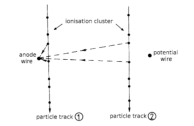
\includegraphics[scale = 2]{pictures/drift_ch_diff_paths.pdf}
\caption{Different drift paths for near\\ and distant particle}
\label{fig:drift_ch_diff_path}
\end{minipage}  
\begin{minipage}[c]{0.5\textwidth}
\centering
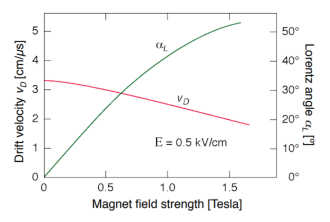
\includegraphics[scale=1]{pictures/lorentz_angle.pdf}
\caption{Lorentz angle and drift velocity in a magnetic field}
\label{fig:lorentz_angle}
\end{minipage}
\end{figure}

Un'altra caratteristica importante associata a camere di questo tipo è l'ambiguità sinistra-destra che emerge quando si tenta di stimare la distanza della traccia della particella dai cavi della camera.
\begin{wrapfigure}{r}{5.5cm}
\caption{Resolution of the left-right ambiguity}
\label{fig:left_right_ambiguity}
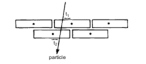
\includegraphics[width=5.5cm]{pictures/drift_ch_left_right.pdf}
\end{wrapfigure} 
Il sistema si limita infatti a misurare un intervallo temporale, e pertanto in nessun modo può distinguere se la radiazione sia passata a destra o a sinistra del cavo. Solitamente si mantiene l'ambiguità andando a individuare due punti, uno "vero" (legato al passaggio della particella) e uno "fantasma", che dovrà essere escluso, e la si risolve apportando delle modifiche alla camera e aggiungendo un secondo livello di celle, sfalsato rispetto al primo (come mostrato in figura \ref{fig:left_right_ambiguity}). Unendo le informazioni dei due livelli è possibile distinguere i punti che effettivamente corrispondono alla traccia della particella, in quanto sono gli unici allineati, risolvendo così l'ambiguità del sistema.\\ 


\begin{figure}[hbtp]
\centering
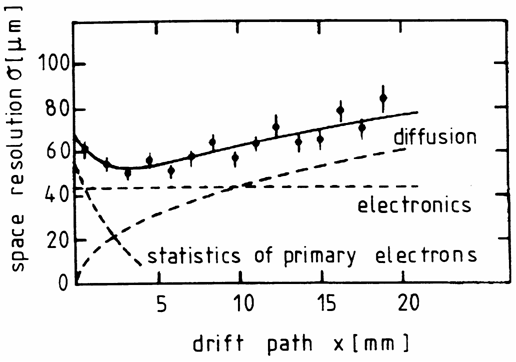
\includegraphics[scale=1.5]{pictures/drift_chamber_resolution.pdf}
\caption{Spatial resolution in a drift chamber as a function of the drift path}
\label{fig:drift_resolution}
\end{figure}


\chapter{Muons}

\section{About the Particle}
I \textit{muoni} sono fermioni fondamentali, attualmente calssificati come leptoni, largamente utilizzati dal punto di vista sperimentale, grazie sopratutto ai modi in cui questi interagiscono con la materia. Hanno una vita media abbastanza elevata rispetto ad altre particelle subatomiche, dovuta al fatto che il loro decadimento è mediato dall'interazione debole, le cui tempistiche sono 
molto più larghe rispetto, per esempio, all'interazione forte, di cui i muoni non risentono. Inoltre, grazie alla massa elevata, vengono decelerati in maniera meno significativa in presenza di campi elettromagnetici, perdendo meno energia a causa di fenomeni come ionizzazione o irraggiamento e quindi arrivando anche a grandi profondità nei materiali che attraversano.\\
Un altro vantaggio apportato dall'utilizzo sperimentale dei muoni è la facilità con cui è possibile reperirli: tali particelle sono infatti tra i costituenti maggioritari dei raggi cosmici secondari (originati, quindi, in seguito all'interazione con l'atmosfera) che costantemente "bombardano" la Terra.\\
Come accennato in precedenza, la maggior parte dei muoni ha origine cosmica: questi leptoni nascono, infatti, in seguito al decadimento dei pioni prodotti grazie all'interazione tra i raggi cosmici primari e l'atmosfera terrestre, secondo le reazioni:
\[ \pi^- \to \mu^- + \bar{\nu_\mu} \qquad \pi^+ \to \mu^+ + \nu_\mu \]
In laboratorio i muoni possono essere prodotti nei collider, inviando un fascio di protoni ad alta energia (\textgreater 500 MeV) contro un bersaglio di Carbonio o Berillio, generando dei pioni, che poi decadono.

Di seguito si riportano i valori ufficiali associati alle principali grandezze che caratterizzano la particella.\\


\begin{table}[htbp]
\centering
\begin{tabular}{c c}
\textbf{Mass} & $105.6583745(24) (MeV/c^2)$\\
\textbf{Mean Lifetime} & $2.1969811(22) (\mu s)$\\
\textbf{Spin} & $1/2$\\
\textbf{Electric Charge} & $-1 (e)$\\
\textbf{Color Charge} & $Colorless$\\
\textbf{Antiparticle} & $\mu^+ (antimuon)$\\
\textbf{Decay products} & $e^-,e^+,\nu_e,\bar{\nu_e}$\\
\end{tabular}
\caption{Main characteristics of the muon $\mu^-$}
\label{tab:muon_parameters}
\end{table}


\section{Interactions of muons with matter}

Le interazioni principali a cui i muoni vanno incontro quando attraversano un dato materiale, sono essenzialmente di quattro tipologie: 
\begin{itemize}
\item \textbf{Ionization}
\item \textbf{Bremsstrahlung}: cessione, da parte di particelle cariche veloci, quando queste decelerano in presenza del campo coulombiano di un nucleo, di una frazione della loro energia cinetica sotto forma di un fotone. Detta \textit{energia critica} il valore corrispondente alla configurazione in cui le principali perdite di energia (ionizzazione e irraggiamento) si equivalgono, per i muoni tale quantità è stimata intorno agli 890 GeV, oltre i quali questo è l'effetto prevalente.
\item \textbf{Pair production}: in maniera analoga al caso dei fotoni, per muoni sufficientemente energetici si può osservare la scomparsa degli stessi e la conseguente produzione di una coppia $e^+/e^-$, come schematizzato dalla reazione:
\[ \mu + nucleus \to e^+ + e^- + nucleus \]
\item \textbf{Photonuclear interactions}: ad energie molto elevate ( > 10 TeV) cominciano ad assumere importanza anche le collisioni anelastiche muone-nucleo che, dal punto di vista dei detector, possono generare degli "hadronic background" ovvero la rilevazione della presenza di jet di adroni.
\end{itemize}

\subsection{Ionization}
Le particelle cariche, come per l'appunto i muoni, quando attraversano un materiale perdono una certa frazione di energia che cedono agli elettroni degli atomi costituenti, a causa di interazioni di natura elettromagnetica.\\
Tale perdita di energia è esplicitata, per unità di lunghezza, dalla formula di Bethe-Bloch (\ref{eq:Bethe-Bloch}):
\begin{equation}
-\frac{dE}{dx} = \left(\frac{ze^2}{4\pi\varepsilon_0}\right)^2\frac{4\pi Z\rho N_A}{Amv^2}\left[\ln\left(\frac{2mv^2}{I}\right)-\ln(1-\beta^2)-\beta^2\right]
\label{eq:Bethe-Bloch}
\end{equation}
Dove $v$ è la velocità della particella incidente, $z$ la sua carica, $\beta = v/c$, $m$ è la massa dell'elettrone e $A,Z,\rho$ sono le caratteristiche fisiche del materiale attraversato. Infine, $I$ è l'energia media necessaria a ionizzare un atomo del mezzo.\\
L'equazione \ref{eq:Bethe-Bloch} è valida solo per particelle cariche, più massive dell'elettrone e con una velocità abbastanza superiore di quella degli elettroni atomici, anche se ad energie troppo alte entrano in gioco correzioni relativistiche e altri tipi di interazioni. Come ci si aspetterebbe, il grosso della perdita di energia lo si ha a basse velocità, quando l'espressione va come $\sim 1/\beta^2$ (come si osserva in figura \ref{fig:energy_loss_in_air}.\\
\begin{figure}[hbtp]
\centering
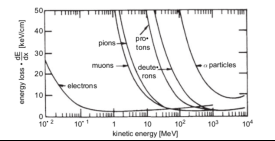
\includegraphics[scale=2]{pictures/particle_energy_loss_in_air.pdf}
\caption{Energy loss for typical particles in air}
\label{fig:energy_loss_in_air}
\end{figure}

Si ricordi comunque che la formula di Bethe-Bloch non permette di calcolare l'energia persa \textit{esattamente} dalla particella, ma rappresenta una perdita media di energia attraverso un materiale, causata da interazioni il cui numero va trattato in maniera statistica. Questo si verifica sopratutto quando si trattano assorbitori sottili, in cui si osservano importanti fluttuazioni dell'energia persa. In questi casi, infatti, la distribuzione della perdita energetica è fortemente asimmetrica, tanto da poter essere rappresentata da una \textit{Distribuzione di Landau}.\\
\begin{wrapfigure}{r}{5.5cm}
\label{fig:landau_distribution}
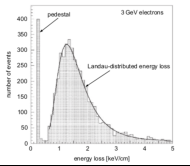
\includegraphics[width=5cm]{pictures/landau.pdf}
\caption{Energy-loss distribution of 3 GeV electrons in a thin-gap drift chamber
filled with Ar/CH 4}
\end{wrapfigure}
 Analiticamente:
\begin{equation}
\label{eq:landau}
L(\lambda) = \frac{1}{\sqrt{2\pi}}\exp\left[-\frac{1}{2}(\lambda+e^{-\lambda})\right]
\end{equation}
dove $\lambda$ rappresenta la deviazione dalla più probabile energia persa:
\[ \lambda = \frac{\Delta E - \Delta E^W}{\xi} \]
con $\Delta E$ che è l'energia effettivamente persa dalla particella in un assorbitore di spessore $x$, mentre $\Delta E^W$ è il corrispondente valore più probabile previsto dalla teoria. $\xi$, invece, corrisponde ad una serie di fattori moltiplicativi ottenibili integrando la formula di Bethe-Bloch.\\

\bigskip
Per quanto riguarda i \textit{range}, ovvero la distanza percorsa all'interno di un dato materiale da una particella prima che questa perda tutta la sua energia, nel caso dei muoni si può stare tranquilli: come spiegato in precedenza, sono leptoni che interagiscono molto poco con la materia, e lo fanno principalmente perdendo energia per ionizzazione. Nel caso, in particolare, dei muoni cosmici, che non vengono prodotti con energie elevatissime (solitamente qualche GeV), gli effetti secondari sono ancora più trascurabili.

\begin{figure}[hbtp]
\begin{minipage}[c]{0.5\textwidth}
\centering
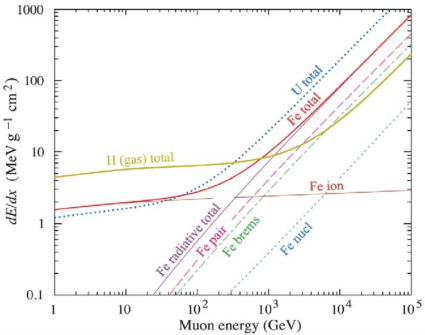
\includegraphics{pictures/muon_energy_loss.pdf}
\caption{Average energy loss of a muon in \\hydrogen, iron, and uranium as a function \\of muon energy.}
\label{fig:muon_energy_loss}
\end{minipage}  \hfill
\begin{minipage}[c]{0.5\textwidth}
\centering
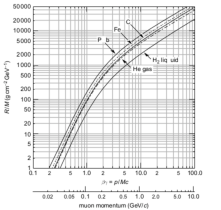
\includegraphics[scale=1.8]{pictures/muon_range.pdf}
\caption{Range of muons in liquid hydrogen, helium gas, carbon and lead}
\label{fig:muon_range}
\end{minipage}
\end{figure}

Come si evince, per esempio, dalla curva corrispondente all'idrogeno gassoso in figura \ref{fig:muon_energy_loss}, fino a qualche centinaio di GeV di energia, l'unico effetto significativo che contribuisce a "rallentare" i muoni è la ionizzazione.\\






\part{LEMMA}

\chapter{Experimental setup}

\section{LEMMA}

L'esperimento nasce nell'ambito del progetto LEMMA (che sta per Low Emittance Muon Accelerator), che consiste in un particolare tipo di approccio sviluppatosi negli ultimi anni per lo studio di queste particelle.\\
Come noto, l'utilità dei collider di muoni nello sviluppo di nuova fisica è veramente molto alta: innanzitutto in quanto particelle elementari (a differenza, per esempio, dei protoni), quando questi costituiscono un fascio tutta l'energia ed il momento sono disponibili, in assenza di interazioni tra i sottosistemi; inoltre, la massa maggiore rispetto ad altre particelle elementari riduce la perdita di energia per radiazione di sincrotrone.\\
Il problema sussiste però nella costruzione di questi fasci. Producendo muoni in maniera "tradizionale", ovvero sfruttando collisioni di adroni energetici contro dei target, si ottengono fasci con una \textit{emittance} (dispersione) troppo elevata, costituiti quindi da particelle troppo poco localizzate, tanto da necessitare di un \textit{cooling}, di un raffreddamento prima di essere utilizzati. Il problema di questo processo è che richiede tempo, durante il quale i muoni rischiano di decadere.\\
Un \textit{low emittance particle beam} è un fascio in cui le particelle sono confinate a piccole distanze fra di loro e hanno tutte più o meno lo stesso impulso, ed è quindi "già pronto" ad essere utilizzato in un collider o un anello di accumulazione. Per ottenere un fascio di questo tipo si sfruttano gli urti tra dei positroni inviati contro un target e gli elettroni a riposo di quel bersaglio. Il vantaggio più grande apportato da questa soluzione consiste nel fatto che le coppie $\mu^+/\mu^-$ prodotte sono "confinate" in una regione molto ristretta, limitata sia longitudinalmente, sia trasversalmente.\\
Riassumendo, pertanto il progetto LEMMA permette la costruzione di fasci di muoni a bassa \textit{emittance}, localizzati spazialmente e che non necessitano di interventi di cooling. Tutto ciò consente quindi di lavorare con un'elevata efficienza di raccolta (meno muoni che decadono) e un minor numero di eventi di fondo, a spese di una minore cross-section che implica un minor numero di muoni prodotti, rispetto ad altre tecniche.\\


\section{Test beam setup}

Il setup sperimentale consiste in 4 camere a drift, una rivisitazione di quelle usate dentro CMS per rilevare i muoni. Il sistema è stato riprodotto a Legnaro nel 2018, ed è attualmente utilizzato nella raccolta dati volta alla ricostruzione delle tracce dei muoni cosmici.\\
Il progetto nasce inizialmente come test beam, per studiare fasci di muoni, valutandone le caratteristiche ad esempio, per stabilire se questi fossero pronti per essere usati in un collider. In particolare, veniva analizzata la produzione di coppie $\mu^+/\mu^-$ ad opera di un fascio di positroni a 45 GeV inviato contro un target di Berillio.\\
Lo schema del primo apparato costruito (2018) è riportato in figura \ref{fig:lemma_test_beam_2018}, di cui le 4 camere a drift costituiscono solo la parte finale (le linee in celeste).\\
\begin{figure}[hbtp]
\centering
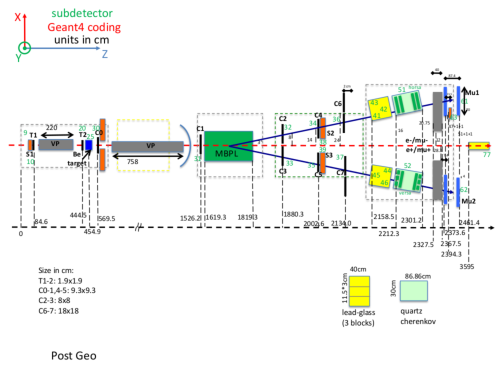
\includegraphics[width=\textwidth,height=0.4\textheight]{pictures/lemma_2018.pdf}
\caption{Experimental setup used for test beam in 2018}
\label{fig:lemma_test_beam_2018}
\end{figure}


Per quanto riguarda le camere, si ha che ciascuna di esse è costituita da 4 livelli di tubi di drift, i quali contengono ognuno 16 celle, di dimensioni 42 x 13 (mm), al centro di cui un cavo metallico funge da anodo, mentre le pareti da catodo. Il campo elettrico all'interno va come 1/r, dove r è la distanza dal centro della cella, e attira pertanto gli elettroni di ionizzazione prodotti in seguito al passaggio di un muone attraverso il gas contenuto nel detector ( $85\%$ Ar e $15\%$ CO\ped{2}). Poichè la velocità degli elettroni all'interno del gas è costante, grazie ad un sistema di elettronica che misura il tempo di arrivo della prima ionizzazione, è possibile ricostruire la posizione in cui è passato il muone rispetto al centro della cella (sempre con la left-right ambiguity rappresentata in figura \ref{fig:left_right_ambiguity}). Combinando le informazioni di tre o quattro celle consecutive su layer differenti è possibile risolvere la left-right ambiguity e ricostruire la traccia locale della particella; noti poi i punti che costituiscono la traccia locale, non è difficile processare la traccia "globale", quella che effettivamente delimita il percorso del muone attraverso le camere. Un esempio di traccia proveniente da un file di calibrazione (costituito cioè di muoni singoli prodotti appositamente per calibrare l'apparato), raccolto nel 2018, è riportato in figura \ref{fig:example_track_2018}.\\

\begin{figure}[hbtp]
\centering
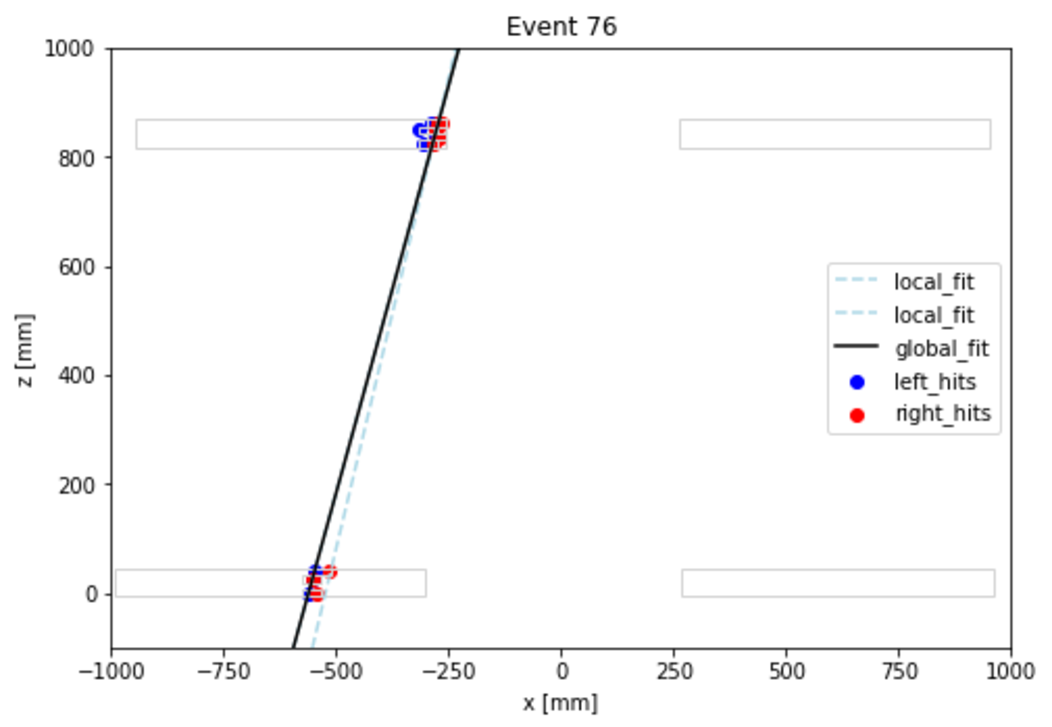
\includegraphics[scale=0.4]{pictures/2D_example_global.pdf}\hfill
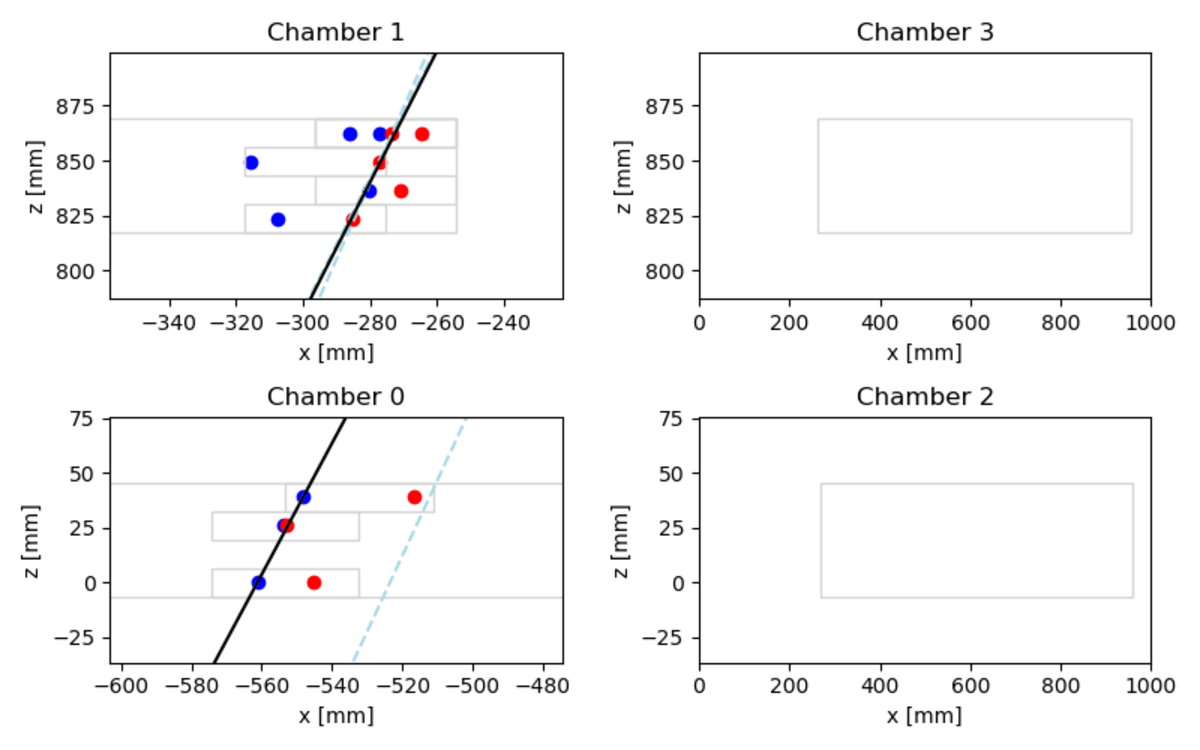
\includegraphics[scale=0.4]{pictures/2D_example_chambers.pdf}
\caption{Track recostruction in 2-dimensional setup (2018)}
\label{fig:example_track_2018}
\end{figure}

L'evento mostrato in figura \ref{fig:example_track_2018} è un evento abbastanza "pulito", nel senso che non si osservano altri segnali, al di fuori di quelli utilizzati per il fit, cosa che purtroppo non succede spesso.\\
Si noti che, come nella maggioranza degli eventi, tracce locali e globali non coincidono perfettamente:  la causa risiede sia nelle imprecisioni del sistema di acquisizione, sia in questioni di sensibilità degli strumenti coinvolti, senza dimenticare il fatto che i tubi di drift non forniscono informazione sulla posizione nella direzione dei fili.\\

\subsection{Trigger and trigger-less data aquisition}

I dati vengono raccolti da un sistema di elettronica che legge i sensori dei detector a 40 MHz (cioè ogni 25 ns), senza il bisogno di un trigger esterno, e vengono registrati ogni volta che almeno un hit viene rilevato da una cella. Sarà quindi l'algoritmo a dover distinguere tra hit corrispondenti ad un segnale e hit dovuti al rumore dell'elettronica.\\
Nel sistema è inoltre presente un dispositivo hardware che ha implementato un algoritmo di mean-timer, ovvero che in automatico riconosce un parziale allineamento nelle celle e lancia un segnale analogo a quello di un sistema di trigger, marchiando come "probabilmente buono", l'evento in cui ha osservato tale allineamento.\\
L'elettronica registra i dati grezzi in formato esadecimale, e li "traduce" direttamente in formato csv. Ciascuna riga del file è formattata allo stesso modo, e contiene sei campi, che identificano in maniera univoca l'hit descritto, e permettono di risalire alla posizione di passaggio della particella.\\

Per motivi che tutt'ora non sono ben chiari, gli esperimenti svolti con questo setup sperimentale (ma anche per quelli successivi) sono stati caratterizzati da un forte rumore (di natura prettamente elettronica), inteso come un gran numero di segnali spuri all'interno dei dati. Per questo motivo è necessario che l'algoritmo che elabora i dati raccolti sia poco sensibile a tale rumore, e quindi molto selettivo nell'identificazione degli eventi di segnale.\\
La motivazione principale dietro questa scelta di non utilizzare un trigger esterno risiede proprio nell'elevato rumore che caratterizza queste camere: la ricerca diretta di un allineamento permette, a spese di una elevata efficienza (definita come il rapporto fra i muoni effettivamente rilevati e quelli complessivamente passati attraverso le camere), di lavorare solo su segnali "puliti".\\


\subsection{Cosmic muon setup}
Attualmente (2019), l'apparato strumentale è stato ridisposto rivolgendo le camere verso l'alto in modo da poter intercettare i muoni cosmici. I principi di funzionamento sono esattamente gli stessi, così come il sistema di elettronica: solo la geometria del problema è cambiata, in quanto ora permette anche la ricostruzione tridimensionale delle tracce. Le quattro camere sono ora disposte una sopra l'altra (come in figura \ref{fig:2019_esp_setup}), parallele a due a due, in modo che una coppia di camere registri l'informazione nella direzione $x$, mentre l'altra coppia nella direzione $y$ (la $z$ è la verticale, lungo cui arrivano i muoni).\\

\begin{figure}[hbtp]
\centering
\includegraphics[scale=0.05]{pictures/2019_setup.pdf}
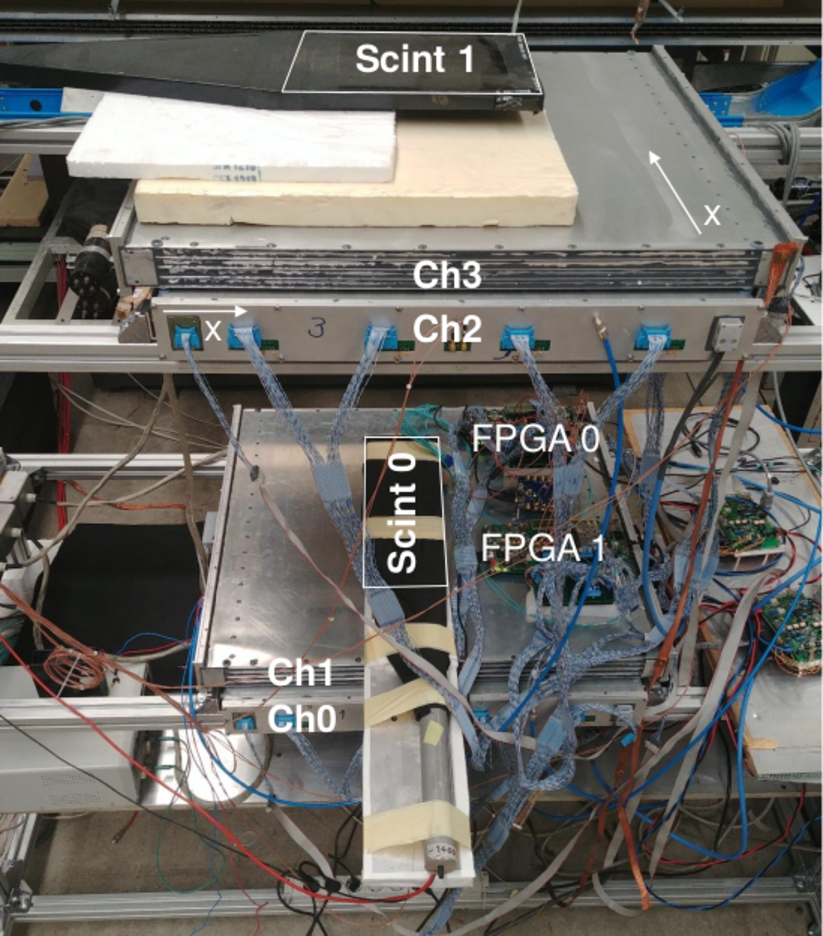
\includegraphics[scale=0.5]{pictures/2019_scint.pdf}
\caption{2019 Experimental setup to spot cosmic muons}
\label{fig:2019_esp_setup}
\end{figure}

La flessibilità dell'apparato, comunque, non impedisce l'istallazione di un vero e proprio sistema di trigger: recentemente, infatti, è stata installata una coppia di scintillatori (figura \ref{fig:2019_esp_setup}). Il vantaggio apportato da degli scintillatori è l'elevata efficienza con cui questi sono in grado di rilevare il passaggio di un muone (prossima al 100\%), a spese della selettività. Inoltre, bisogna tener conto che la superficie dei dispositivi implementati in questo caso, è inferiore rispetto a quella delle camere (circa 1/4), e pertanto non coprono comunque tutto il volume efficace.\\ 
L'utilità principale dell'aggiunta di questi scintillatori risiede comunque nella ricerca di una maggior efficienza e nella possibilità di avere un confronto con i dati raccolti con il firmware di mean-timer.\\
I dati elaborati in questa tesi sono stati raccolti \textit{prima} dell'istallazione di questi scintillatori e pertanto dovranno essere "filtrati" da un opportuno algoritmo che sia in grado di svolgere in maniera efficiente questa analisi \textit{triggerless}.\\

%aggiungere parametri geometrici e/o velocità e tempi di drift?

\chapter{Preprocessing and raw data analysis}

Il sistema di elettronica attualmente in uso registra i segnali delle camere, e li trascrive in un file csv: gli hit contenuti in questo sono codificati mediante 6 campi (HEAD, FPGA, TDC\_CHANNEL, ORB\_CNT, BX, TDC\_MEAS), che permettono di identificare in maniera univoca la camera, il layer e la cella in cui il segnale è stato rilevato. Inoltre, per mezzo di una semplice equazione (riportata in \ref{eq:TIME-NS}), è possibile calcolare il tempo impiegato dall'elettrone di ionizzazione a raggiungere l'anodo.
\begin{equation}
t = ORB\_CNT\cdot3564\cdot25+BX\cdot25+TDC\_MEAS\cdot25/30
\label{eq:TIME-NS}
\end{equation}
Attualmente, non avendo ancora sviluppato un metodo di analisi online, il sistema si limita a salvare file di dati grezzi di 10 MB ciascuno.\\
Questi file vengono per prima cosa processati dall'algoritmo, che ottimizza la memoria occupata (rimuovendo informazioni ridondanti come il campo HEAD del csv, che è uguale per tutti gli hits), costruisce gli eventi e ne effettua una prima e più superficiale selezione.\\
Da questa prima fase di processing viene quindi prodotto un nuovo file comprendente tutti i segnali "accettati", raggruppati in eventi (in base a parametri temporali), pronto per passare alla seconda fase del programma e, in particolare, alla ricostruzione delle tracce.\\

\begin{footnotesize}
Attualmente l'algoritmo gestisce l'analisi degli hits triggerless, ma consente una prima selezione sfruttando il meantimer già implementato nel sistema dell'elettronica. Questo, ma anche eventuali trigger esterni, marchiano gli hits che riconoscono appartenere a eventi di segnale con una speciale sequenza di 64 bit (che compare come una riga nel file csv) contenente le informazioni del trigger che è scattato. Al momento della presa dati l'unico sistema presente era, per l'appunto, quello del meantimer, che viene identificato dal campo TDC\_CHANNEL = 139.\\ L'algoritmo, come accennato, non prevede particolari azioni  sui dati nel caso di trigger esterni (escluso il 139), se non una semplice prima selezione degli hits, ma ne prevede la possibilità.\\
\end{footnotesize}


\section{Recostruction of the events}

La prima (e più semplice) cosa da fare è "completare" il dataframe contentente tutti gli hits, aggiungendo informazioni che permettano una visione più intuitiva del problema, e sostituendo i campi generati dal preprocessing con parametri come la camera, il layer e la cella precisi dove è stato rilevato il singolo segnale. Inoltre è importante anche calcolare (come visto in \ref{eq:TIME-NS}) il tempo intercorso tra il passaggio effettivo della particella e la ricezione del segnale elettronico (in seguito si vedrà che non è proprio così, e che sarà necessario correggere questo parametro).\\
È proprio questo valore temporale a permettere un raggruppamento degli hits in veri e propri eventi di segnale: i muoni cosmici arrivano a terra con velocità molto elevate (stimate intorno ai 30 cm/ns %mettere riferimento?
), e pertanto, per percorrere trasversalmente una delle camere (spessa non più di 6/7 cm) ci impiegano soltanto qualche frazione di nanosecondo, un tempo molto minore di quello impiegato per raccogliere gli elettroni di ionizzazione. Per quanto riguarda questi, infatti, è nota la velocità di drift all'interno del gas utilizzato nelle celle, e pertanto, nota la lunghezza di queste, si ricava un altro parametro di grande importanza per questo apparato, ovvero il massimo tempo di deriva impiegato per raccogliere le cariche prodotte praticamente a bordo cella, che è stimato a 390 ns.\\
Proprio grazie a questo parametro è possibile raggruppare temporalmente gli hits, "dando il tempo di essere viste" anche alle cariche prodotte a distanza maggiore dall'anodo. Dal punto di vista tecnico, ciò consiste nel richiedere che hits consecutivi nel dataframe, che distano temporalmente meno del 110\% del tempo massimo di deriva (si considera un pochino di più per tener conto della precisione dei clocks utilizzati), facciano parte dello stesso evento.\\
Un tale discriminante è necessario: se l'elettronica legge i detector ogni 25 ns, non si può sperare di aver raccolto tutta la carica in un così breve lasso di tempo, ma si devono unire le informazioni raccolte su più acquisizioni.\\

Infine si impone una prima condizione sugli eventi appena costruiti: che questi siano costituiti di almeno 6 hits differenti. La motivazione risiede nell'elevata presenza (emersa osservando i dati grezzi) di numerosi eventi con 1 o 2 segnali soltanto, che palesemente non rappresentano nulla di fisico ma sono puramente rumore elettronico. Sei hits sono poi il minimo numero di punti che in seguito sarà richiesto per costruire un fit a livello globale, unendo due fit locali che, come accennato in precedenza, necessitano di almeno 3 punti ciascuno.\\


\section{Time Pedestal}

Il prossimo passo consiste nella stima della distanza esatta dal cavo a cui sono passate le particelle, calcolabile una volta noto il tempo di drift degli elettroni prodotti, sfruttando la relazione \ref{eq:POSITION}:
\begin{equation}
x = v_d\cdot(t-t_0)
\label{eq:POSITION}
\end{equation}
Dove $t_0$ è un opportuno parametro, detto \textit{time pedestal}, che contiene contributi dovuti alla latenza del trigger (assente, in questo caso), e al tempo necessario all'elettronica per rilevare e raccogliere i dati.  La velocità di drift $v_d$ viene invece assunta costante all'interno della cella.\\
Eventuali correzioni a questi due parametri verranno effettuate durante la fase di calibrazione.\\

In un detector ideale, le misure temporali dei segnali raccolti seguirebbero una distribuzione uniforme tra 0 ns (passaggio in corrispondenza del'anodo) e 390 ns (passaggio sul bordo della cella). Nella pratica, però, sono presenti inevitabili ritardi nei segnali dovuti a latenza nei sistemi di trigger, oppure semplicemente alla lunghezza dei cavi collegati all'elettronica di front-end, che contribuiscono al tempo misurato (TIME\_NS) come segue:
\[ TIME\_NS = t_{drift} + t_0^{wire} + t_{trigger} \]
Questi contributi secondari vengono solitamente corretti mediante dei test di calibrazione o delle analisi sulle distribuzioni temporali, riadattando le misure in maniera tale che seguano la distribuzione uniforme prevista.\\

Ma ecco che entra in gioco un altro vantaggio apportato dall'utilizzo di camere di deriva costruite in questa maniera: si sfrutta la geometria con cui sono stati istallati i vari layer di celle (sfasati di mezza cella l'uno dall'altro) per esplicitare un set di equazioni di mean timer grazie al \textit{Teorema di Talete}, che permettono di computare questo time pedestal durante la costruzione stessa degli eventi. \\
Dal punto di vista pratico il teorema è applicabile andando a cercare degli opportuni pattern di allineamento all'interno della singola camera del singolo evento, un esempio dei quali è riportato in figura \ref{fig:alignment_pattern}, ed è risolto dall'equazione \ref{eq:t0_pattern} (nella quale, si ricordi, ogni tempo misurato $t_i$ è definito a meno di una costante, $t_i = t_i + t_0$, uguale per tutti i punti), dove $T_{MAX}$ è il massimo intervallo di tempo in cui tutta la carica di ionizzazione è raccolta, e che è  stimato a 390 ns.

\begin{figure}[hbtp]
\begin{minipage}[c]{0.5\textwidth}
\centering
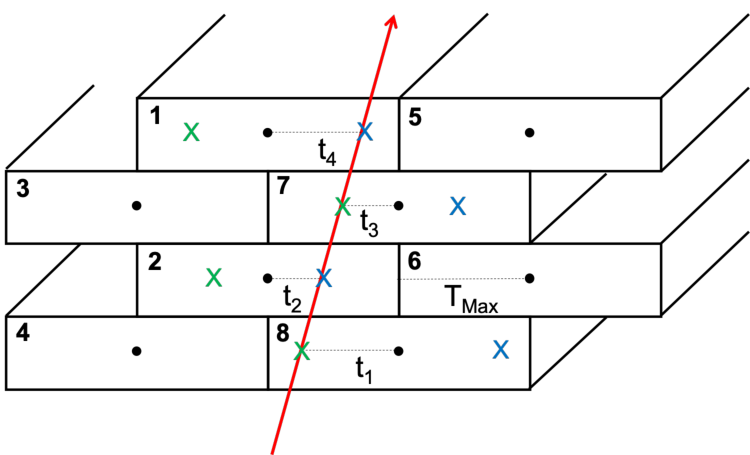
\includegraphics[scale=0.5]{pictures/scheme_track_chamber.pdf}
\caption{Possible pattern for a mean timer equation}
\label{fig:alignment_pattern}
\end{minipage}  
\begin{minipage}[c]{0.5\textwidth}
\begin{align}
T_{MAX} & = \frac{t_1+t_3}{2} + t_2 = \nonumber \\
	        & = \frac{(t_1 + t_0) + (t_3 + t_0)}{2} + (t_2 + t_0) \nonumber \\
& \nonumber\\
t_0 &= \frac{t_1 + t_3 + 2\cdot t_2 - 2\cdot T_{MAX}}{4} \label{eq:t0_pattern}
\end{align}
\end{minipage}
\end{figure}



In realtà, ogni cella avrebbe il suo specifico $t_0$, ma le differenze tra la varie celle sono dell'ordine di qualche ns al più, e quindi trascurabili in prima approssimazione. Per questo motivo l'algoritmo procede nel seguente modo:
\begin{itemize}
\item[-] Raggruppa i dati per singoli eventi, ed effettua una prima selezione eliminando tutti gli eventi che contengono meno di due camere con punti in almeno 3 layers differenti (cioè la configurazione minima per costruire, in seguito, una traccia).
\item[-] Presi singolarmente gli eventi, effettua un'ulteriore suddivisione degli hits in base alla chamber a cui questi appartengono, passandoli, poi, al vero e proprio algoritmo di mean timer.
\item[-] Senza entrare troppo nel tecnico, l'algoritmo combina le celle presenti nella camera, in cui è stato rilevato il segnale, in tutte le combinazioni possibili di 3 elementi, riconosce le triplette a cui è possibile applicare il teorema di Talete e calcola il relativo time pedestal risolvendo un'equazione di mean timer analoga a quella scritta in \ref{eq:t0_pattern}.
\item[-] Nel caso (abbastanza frequente) in cui nella stessa chamber compaiano più pattern risolvibili, l'algoritmo calcola tutte le stime di $t_0$ del caso, e semplicemente ne fa una media. 
\item[-] La stima (media o no) così trovata del time pedestal viene estesa a tutti gli hits che fanno parte di uno degli allineamenti trovati dal programma, permettendo una corretta stima del loro tempo effettivo di deriva. Inutile specificare che tutti i punti non facenti parte di alcun pattern sono stati esclusi dal dataframe complessivo.
\end{itemize}

% mettere altri pattern di esempio?

Noto, a questo punto, l'effettivo drift time degli elettroni per ogni singolo hit, è banale calcolare il punto in cui il muone è passato, con la relazione cinematica: $x = v_d(t - t_0)$ (con $v_d$ velocità di drift delle cariche nel gas e $t$ misura temporale dell'elettronica). Si ricordi che ancora non è stata risolta la left-right ambiguity, e che pertanto la $x$ appena trovata determinerà due punti nella cella, e non uno soltanto.\\
Un ultima selezione viene effettuata rimuovendo gli hits con un valore "non fisico" di posizione, ovvero i punti che appaiono "fuori dalla cella" in cui sono stati trovati, con un valore di $x$ minore di 0 o maggiore di 21 mm (lunghezza della cella).\\

A questo punto si può verificare l'efficacia del metodo, andando a valutare le distribuzioni dei tempi di deriva misurati e quelli computati. L'attesa è una distribuzione uniforme tra 0 e 390 ns, ovvero i valori possibili considerando le dimensioni della singola cella e la velocità di deriva degli elettroni.

\begin{figure}[hbtp]
\begin{minipage}[c]{0.5\textwidth}
\centering
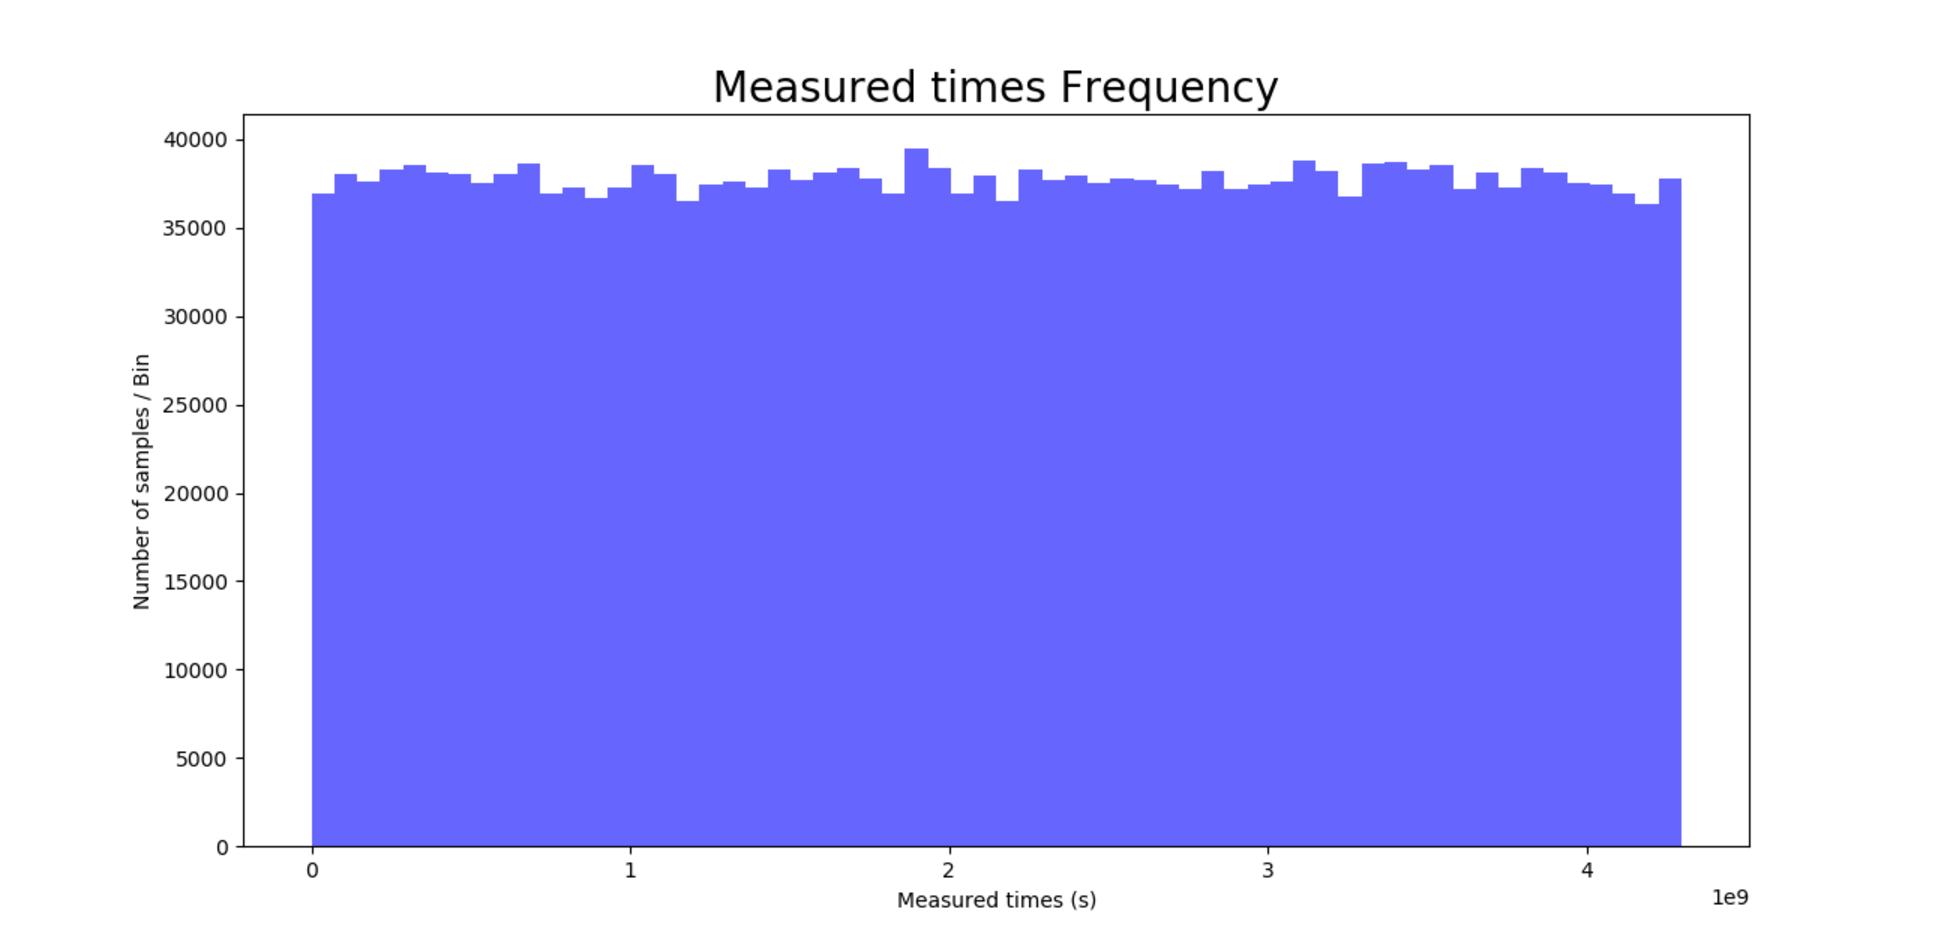
\includegraphics[scale=0.25]{pictures/Measured_times_Frequency.pdf}
\caption{Distribution of measured drift times}
\label{fig:TIME_NS}
\end{minipage}  
\begin{minipage}[c]{0.5\textwidth}
\centering
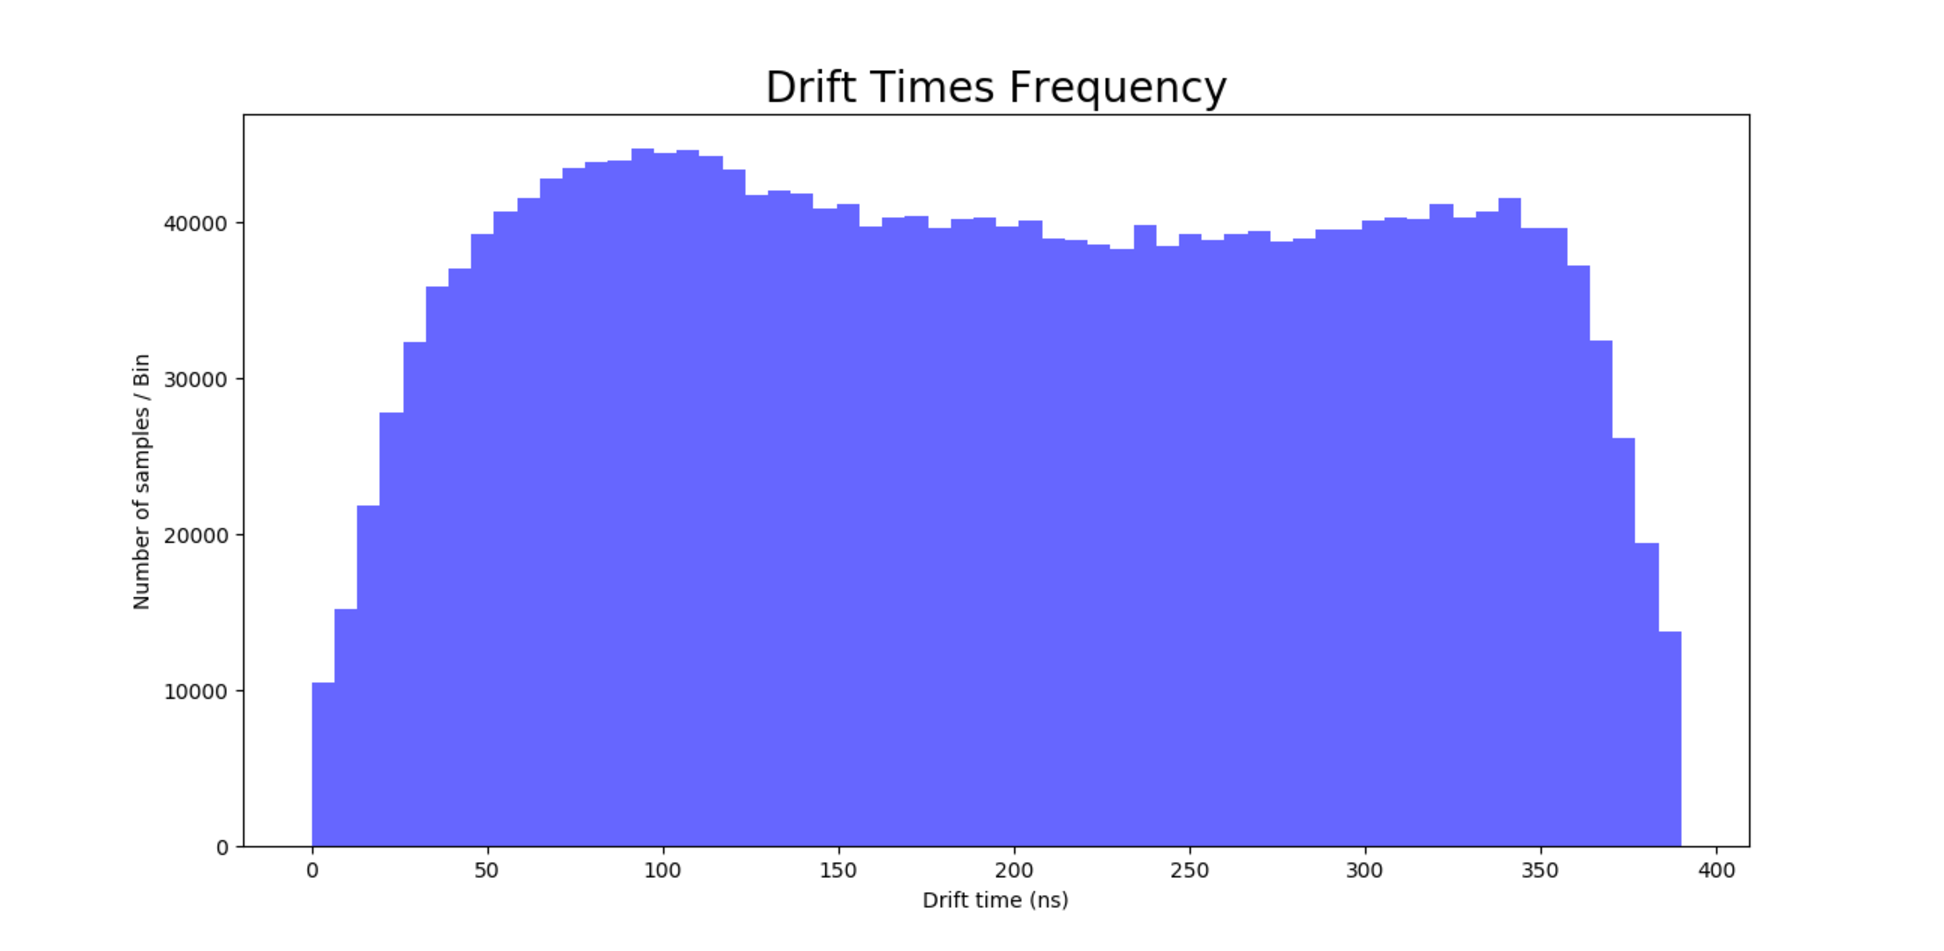
\includegraphics[scale=0.25]{pictures/Drift_Times_Frequency.pdf}
\caption{Final distribution of drift times}
\label{fig:DRIFT_TIMES}
\end{minipage}
\end{figure}

Per quanto riguarda le misure, i risultati sono coerenti con le aspettative, inoltre si vede come la distribuzione sia uniforme tra 0 e un pò più di 400 ns, segno concreto del contributo dovuto a questo time pedestal.  Per quanto riguarda gli effettivi tempi di deriva, invece, la distribuzione presenta delle evidenti irregolarità, che possono essere ricondotte a svariate motivazioni, come l'effetto a cui vanno incontro gli elettroni di ionizzazione a seconda di dove vengono prodotti (descritto in \ref{fig:drift_ch_diff_path}). Un altra probabile ragione è da ricondurre al modo in cui l'algoritmo stesso elabora i tempi di drift: in presenza di più pattern di allineamento nella medesima camera, infatti, viene tenuto conto solo del valor medio dei time pedestal trovati in questa maniera (stime che non è garantito siano compatibili), e ciò avrebbe potuto causare gli effetti spuri che si osservano nel grafico \ref{fig:DRIFT_TIMES}.\\

Il metodo utilizzato resta tuttavia abbastanza efficiente, e i risultati verranno in seguito sottoposti ad una fase di calibrazione per tentare di eliminare le anomalie.\\



\section{Raw data analysis}

È possibile effettuare diverse analisi dei dati raccolti, ancora prima di iniziare a ricostruire le tracce, ancora prima di calibrare lo stesso apparato. Queste analisi preliminari, in genere, comunque, non servono tanto a studiare le caratteristiche fisiche dei muoni che attraversano le camere, quanto a fornire una prima stima dell'efficacia dell'algoritmo e della funzionalità dei vari strumenti, nonchè a fornire una classificazione a priori degli eventi con cui si avrà a che fare.\\
Per prima cosa, si può quantificare l'efficienza di tutti i sistemi di selezione (oltre che dell'algoritmo di mean timer) implementati nel codice: tale analisi, riportata nella tabella \ref{tab:trigger_efficiency} rivela che circa il 90\% dei segnali raccolti appartiene a eventi di fondo. Si dovrebbe essere portati a pensare che la causa di ciò sia un algoritmo eccessivamente selettivo ma, come spiegato in precedenza, il codice si limita a verificare la presenza di pattern di allineamento e ad escludere quelli per cui non viene calcolato un buon tempo di deriva. Pertanto il programma non elimina gli eventi rumorosi, ma solo i segnali isolati. La dicitura \textit{shower} che compare nella tabella, inoltre, si riferisce a quelle "cascate" di particelle che possono formarsi in un rivelatore, e si manifestano con un numero molto grande di segnali nelle varie camere. Tali eventi presentano inevitabilmente delle triplette di allineamento (gli hits sono talmente tanti che occupano quasi tutte le celle in una certa regione) e sono pertanto accettati da questa prima parte di software; rimane impossibile, però, distinguere all'interno di questi delle tracce complete.\\

\begin{table}[htbp]
\centering
\begin{tabular}{c|c}
\toprule
\textit{Total hits detected (signal + background)} & 24494976\\
\midrule
\textit{Total events identified} & 66543\\
\midrule
\textit{Total hits belonging to identified events} & 2265046 (9.25 \%)\\
\midrule
\textit{Showers ( \textgreater 20 hits)} & 1621 (0.60 \%)\\
\midrule
\textit{Showers ( \textgreater 40 hits)} & 139 (0.05 \%)\\
\bottomrule
\end{tabular}
\caption{Selection efficiency of the algorithm}
\label{tab:trigger_efficiency}
\end{table}

Un'altro utile studio emerge valutando l'efficienza delle singole celle: nell'immagine in figura \ref{fig:hit_freq} è rappresentato un grafico bidimensionale contenente le informazioni sulla quantità di segnali (accettati) rilevati da ogni singola cella. Subito saltano all'occhio le celle scure sparse presenti nella camera 0: la causa di questo è nota, e risiede in problemi di natura meccanica. La camera 0 è infatti stata la prima ad essere installata, e in seguito ci si era accorti che alcune celle erano disattivate, e non raccoglievano segnali. Tuttavia, ritenuto uno sforzo inutile smontarla (è la camera situata più in basso e pertanto sarebbe necessario smontare tutto l'apparato), le celle danneggiate sono relativamente poche e perciò non pesano eccessivamente sul risultato finale del lavoro. Le zone più scure a quelle disattivate invece sono una conseguenza dell'algoritmo di mean timer: non trovando segnali in alcune celle, è necessario escludere tutti i pattern che coinvolgono queste. Infine si nota anche una piccola regione meno efficiente nella camera 1, che sembra essere dovuta ad un qualche effetto di schermo parziale che limita il passaggio delle particelle in quella zona.\\

\begin{figure}[hbtp]
\centering
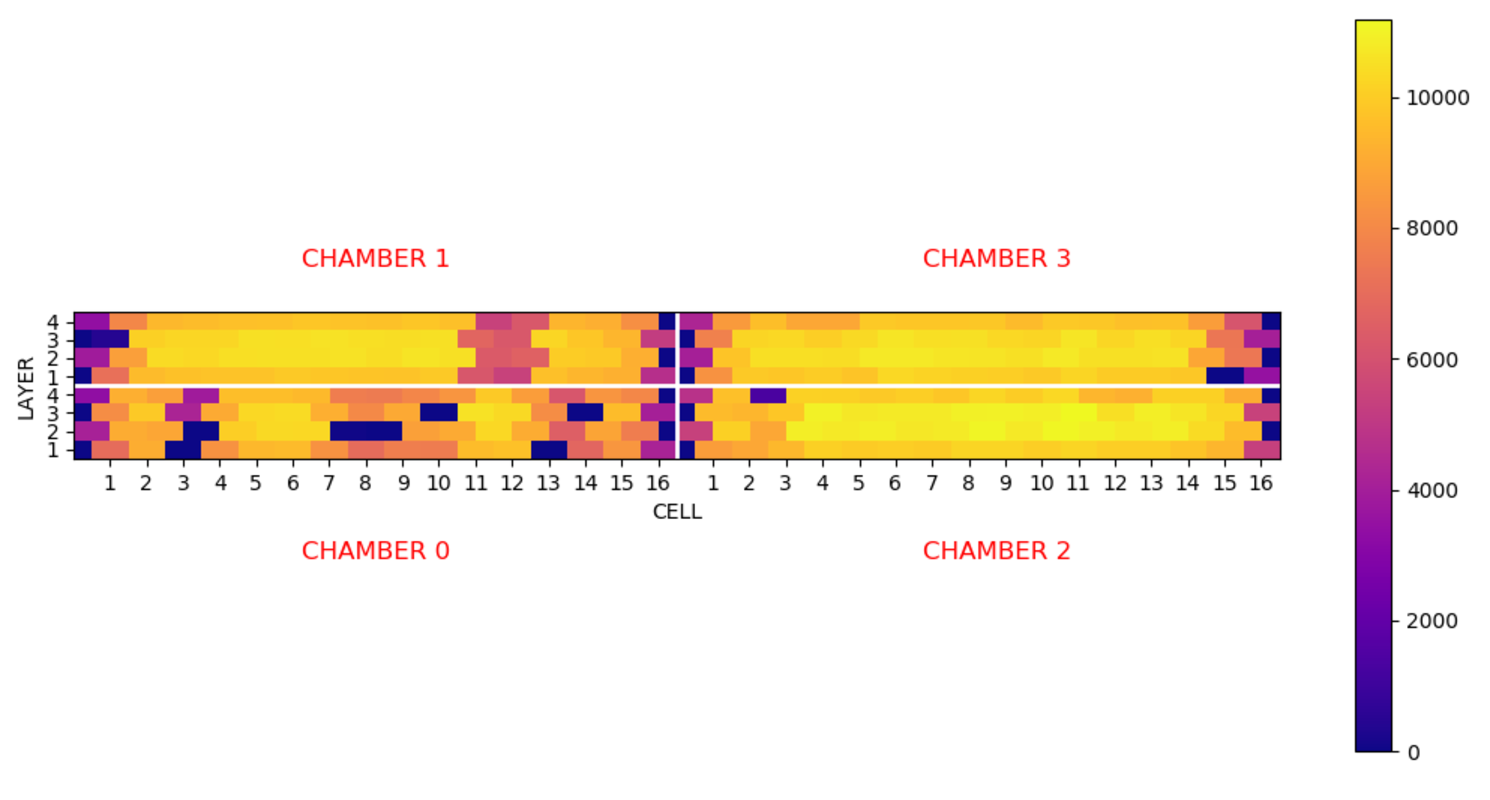
\includegraphics[scale=0.7]{pictures/Hit_matrix.pdf}
\caption{2D representation of hit frequency in the cells}
\label{fig:hit_freq}
\end{figure}

Un altro utile strumento per valutare l'efficienza delle camere può essere il plot bidimensionale del relativo numero di segnali presente fra le coppie di camere (riportati nelle figure \ref{fig:ch1_ch0}, \ref{fig:ch1_ch0_zoom} e \ref{fig:ch3_ch2}). Come si vede nell'immagine zoomata, la maggior parte degli eventi è composta da meno di 10 hits per camera, e si osservano dei picchi in corrispondenza di 3 o 4 hits (in entrambe le camere, ma anche per una sola delle 2) che corrispondono ad un evento di segnale, cioè al passaggio di una particella. In ogni caso, non sono assenti gli eventi costituiti da un numero molto grande di hits, quelli che in tabella \ref{tab:trigger_efficiency} sono classificati come shower. 

\begin{figure}[hbtp]
\begin{minipage}[c]{0.5\textwidth}
\centering
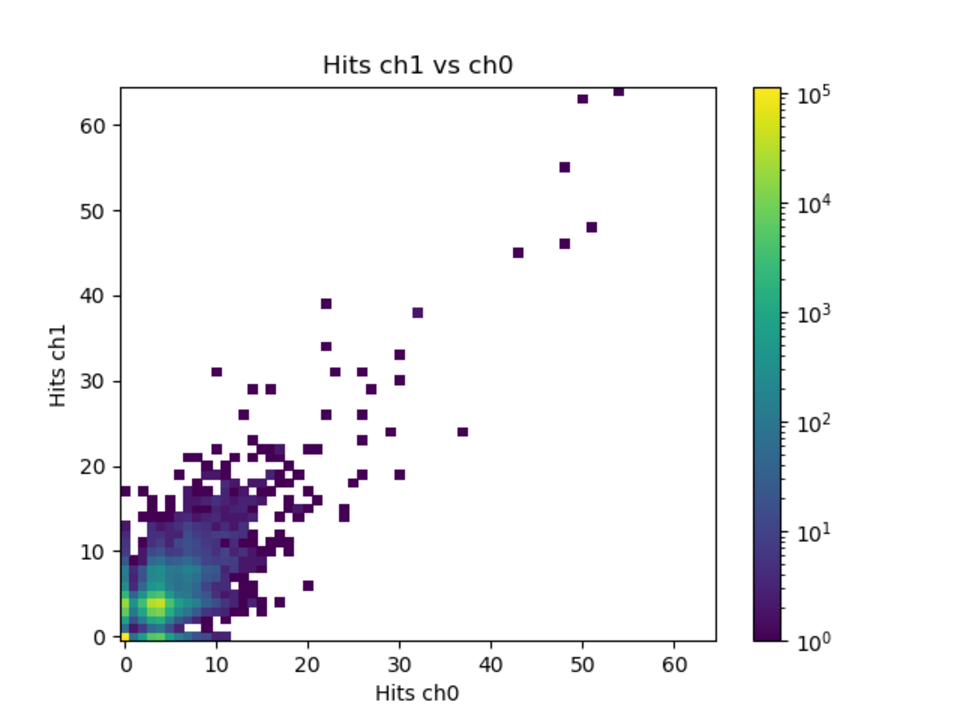
\includegraphics[scale=0.5]{pictures/Hits_ch1_vs_ch0.pdf}
\caption{Hits distribution between chamber 0 and 1}
\label{fig:ch1_ch0}
\end{minipage}  
\begin{minipage}[c]{0.5\textwidth}
\centering
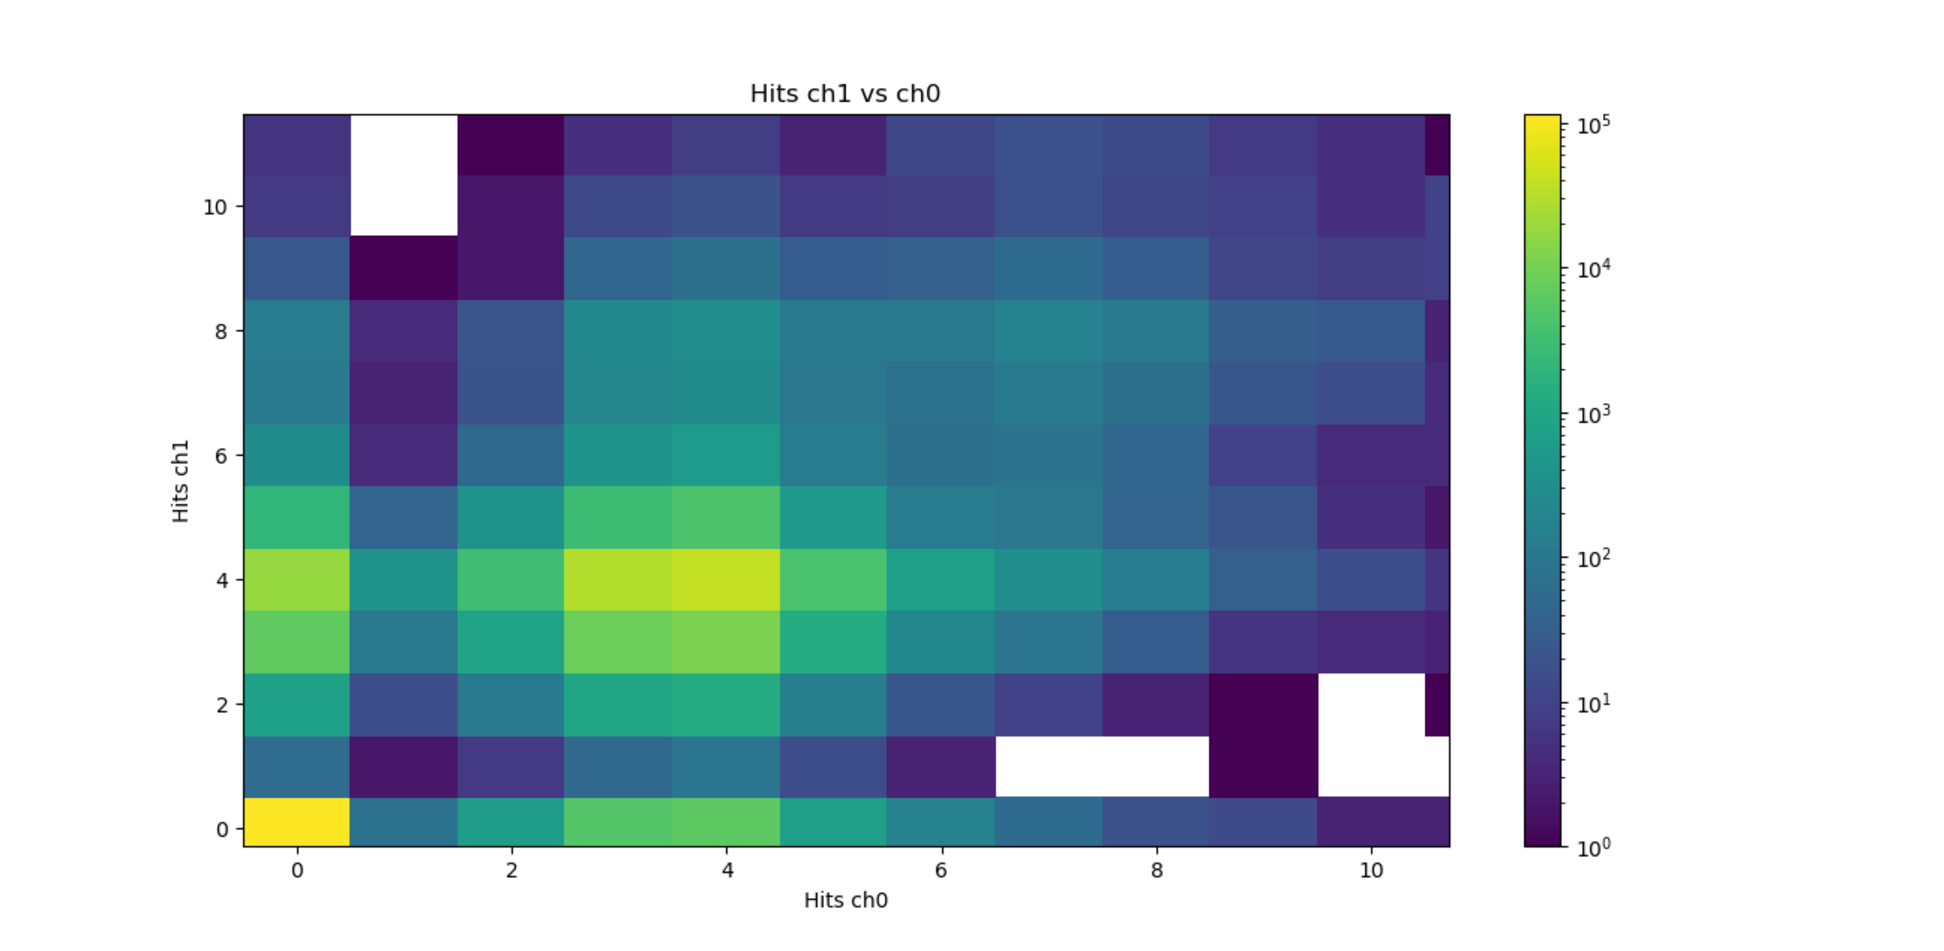
\includegraphics[scale=0.3]{pictures/Hits_ch1_vs_ch0_zoom.pdf}
\caption{Zoomed on events with 10- hits}
\label{fig:ch1_ch0_zoom}
\end{minipage}
\end{figure}

L'operazione si può ripetere anche per valutare l'efficienza dei due dispositivi FPGA (figura \ref{fig:fpga0_fpga1}). Immediatamente si notano le medesime caratteristiche dei grafici che rappresentano le camere: picchi di eventi in corrispondenza di un numero "buono" di segnali (3 o 4 per camera che diventano 7 o 8 nel singolo FPGA) dato che ognuno di questi due dispositivi "vede" la sua coppia di camere (una sopra e una sotto).

\begin{figure}[hbtp]
\begin{minipage}[c]{0.5\textwidth}
\centering
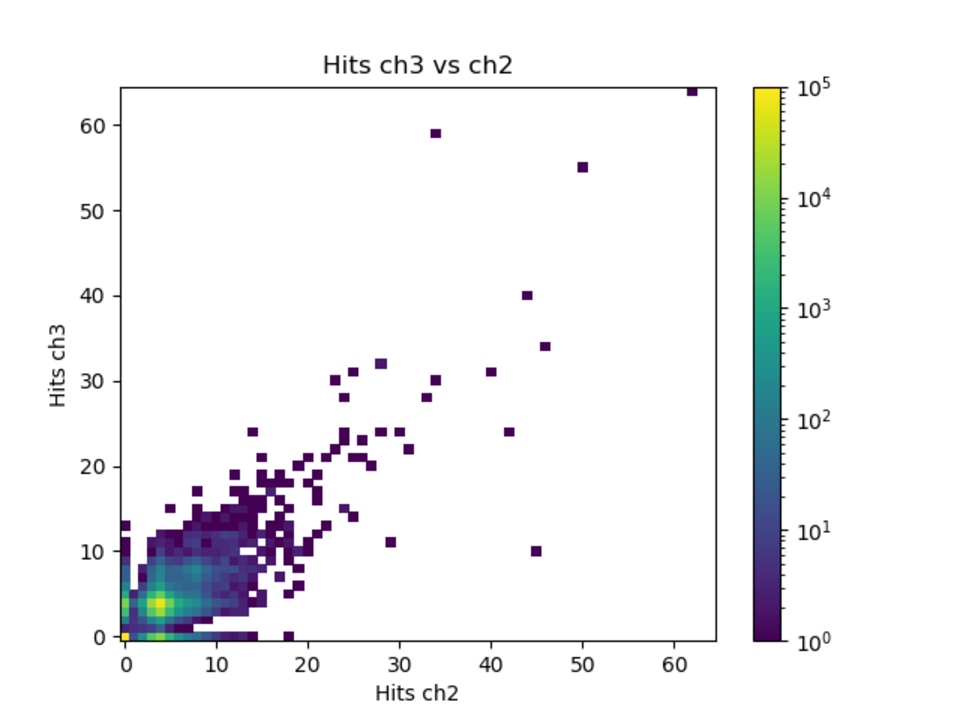
\includegraphics[scale=0.5]{pictures/Hits_ch3_vs_ch2.pdf}
\caption{Hits distribution between chamber 2 and 3}
\label{fig:ch3_ch2}
\end{minipage}  
\begin{minipage}[c]{0.5\textwidth}
\centering
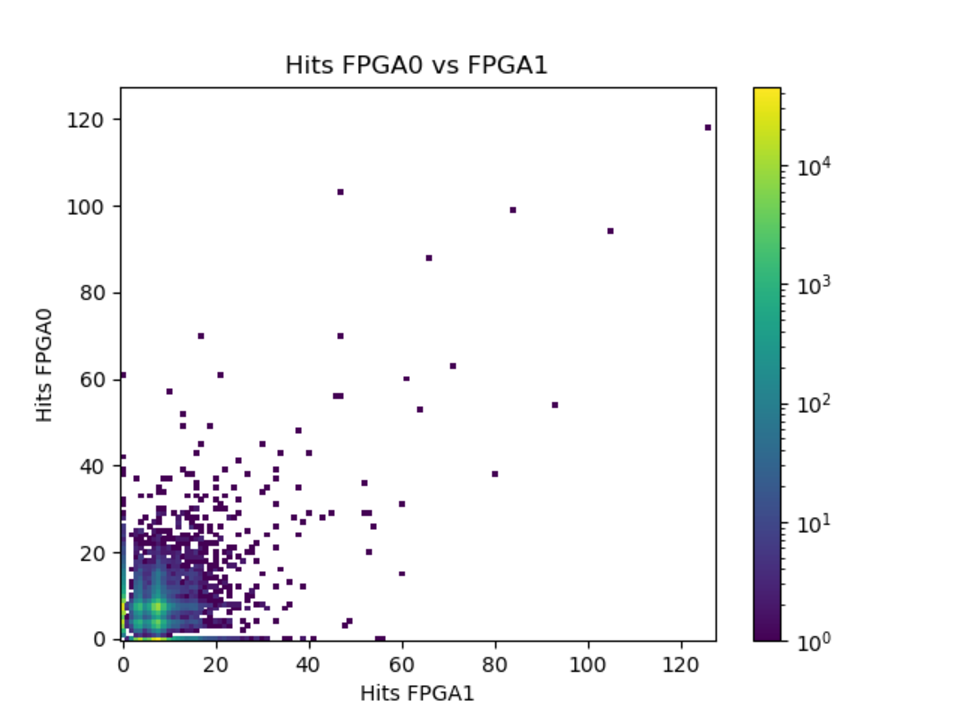
\includegraphics[scale=0.5]{pictures/Hits_FPGA0_vs_FPGA1.pdf}
\caption{Hits distribution between FPGA 0 and 1}
\label{fig:fpga0_fpga1}
\end{minipage}
\end{figure}


Fin'ora si è sempre parlato di un numero "buono" di hit per camera, corrispondente al minimo numero di punti necessario per ricostruire un fit (cioè almeno uno per layer). Come si vede dal grafico \ref{fig:hits_per_event} (dal quale sono stati esclusi i punti troppo rumorosi) la stragrande maggioranza degli eventi selezionati dal meantimer sembra "buona", o almeno presenta un buon numero di allineamenti. Con buona probabilità, infatti, la colonna più alta (con 8 hits) rappresenta un evento di segnale, in quanto 4 punti in 2 camere (una sopra e una sotto) costituiscono una traccia o, almeno, la sua proiezione su uno dei due piani (xz o yz). Ancora più belli sono gli eventi che presentano circa 15-16 hits: nel migliore dei casi sono suddivisi in 4 per camera, costituendo una doppia proiezione, che permette di ricostruire il passaggio del muone in 3 dimensioni.\\
Il picco a 4 hits è invece dovuto al metodo di lavoro dell'algoritmo di meantimer: probabilmente è stato rilevato un allineamento in una delle camere (per cui l'evento è stato comunque costruito), ma i segnali nelle altre sono stati esclusi a causa probabilmente di un mancato allineamento o di un errato computo nella posizione esatta riconducibile ad approssimazioni o un'errata stima del time pedestal.\\

\begin{figure}[hbtp]
\centering
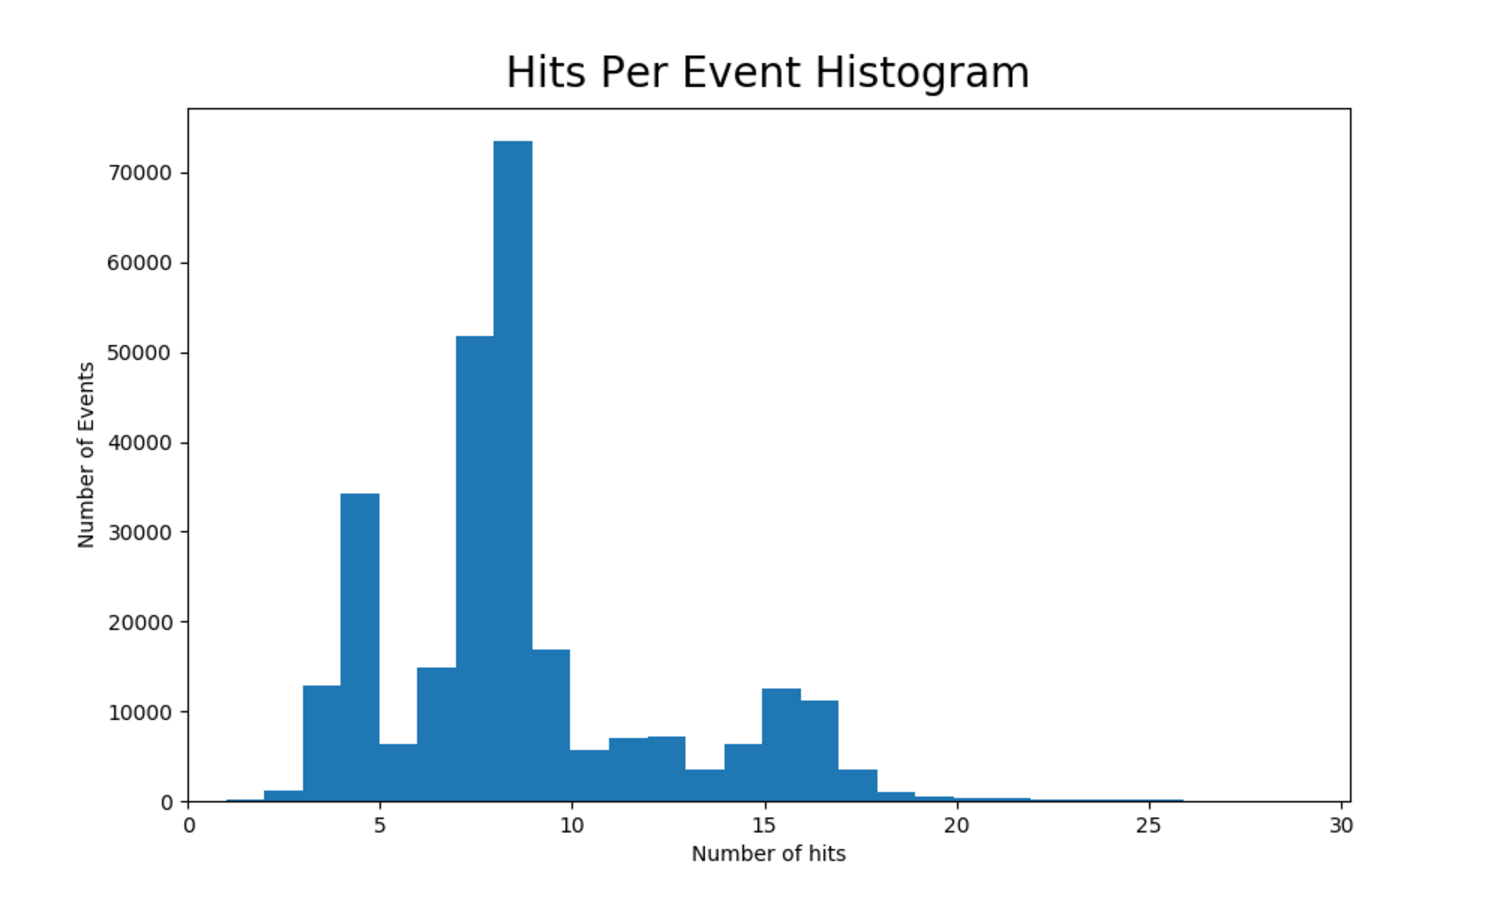
\includegraphics[scale=0.5]{pictures/Hits_per_event.pdf}
\caption{Number event with a certain amount of hits}
\label{fig:hits_per_event}
\end{figure}


Quest'analisi preliminare si può concludere con una prima stima a priori dell'efficienza delle varie camere: richiedendo che una camera "spotti un segnale" quando registra almeno 3 hits in 3 layer differenti si può costruire la tabella \ref{tab:chamber_efficiency}, dove vengono riportate le probabilità condizionate di avere una delle camere della coppia "buona" quando anche l'altra lo è.  In generale, come si vede, i risultati sono abbastanza buoni, nel senso che nella maggior parte dei casi, se una camera vede il muone, l'altra non è da meno. Il problema sorge nei dati che riguardano la camera 0, meno efficiente delle altre. Ma questo problema era già stato riportato in precedenza, ed è riconducibile al mancato funzionamento di alcune delle celle, cosa che, unita al modo in cui funziona l'algoritmo, causa una leggera perdita di segnali.
\begin{table}[htbp]
\centering
\begin{tabular}{c|c}
\toprule
Good\_ch0 $\mid$ Good\_ch1 &  76.42\% \\
\midrule
Good\_ch1 $\mid$ Good\_ch0 &  87.64\% \\
\midrule
Good\_ch2 $\mid$ Good\_ch3 &  89.45\% \\
\midrule
Good\_ch3 $\mid$ Good\_ch2 &  86.60\% \\
\bottomrule
\end{tabular}
\begin{tabular}{c|c}
\toprule
Good\_ch0 $\mid$ Good\_ch2 &  27.41\% \\
\midrule
Good\_ch2 $\mid$ Good\_ch0 &  34.91\% \\
\midrule
Good\_ch1 $\mid$ Good\_ch3 &  30.60\% \\
\midrule
Good\_ch3 $\mid$ Good\_ch1 &  32.89\% \\
\bottomrule
\end{tabular}
\caption{Conditional probability using neighbour chamber as a tag}
\label{tab:chamber_efficiency}
\end{table}

Per le coppie di camere nella tabella di destra, invece, valori tanto bassi delle percentuali possono essere ricondotti al fatto che si stanno considerando detector separati da circa un metro di distanza, mentre le coppie della tabella di sinistra identificano camere direttamente a contatto. Eventuali muoni che incidono nel detector con direzioni troppo "inclinate" rispetto alla verticale possono infatti essere spottati dalle camere più in alto e non in quelle più in basso.\\



\chapter{Tracks recostruction}

Prima di iniziare la parte tecnica, cioè la spiegazione di come vengono ricostruite le tracce, è opportuno entrare  nel dettaglio della configurazione geometrica del sistema.\\
Le camere sono rivelatori di forma quadrata di dimensioni 700x700 mm, disposte una sopra l'altra, come mostrato precedentemente in figura \ref{fig:2019_esp_setup}, e sono orientate, a due a due, nelle direzioni x e y dello spazio. In particolare, le camere 0 e 2 riportano le informazioni nella direzione x, mentre le camere 1 e 3 quelle in direzione y.\\

In questa seconda parte l'algoritmo lavora sul file di eventi prodotto in seguito alla fase di preprocess: un file txt in cui ogni riga ora rappresenta un intero evento (non più un singolo hit) con tutte le coordinate dei segnali raccolti e la left-right ambiguity non ancora risolta. Gli eventi vengono quindi letti riga per riga e riscritti ciascuno in un dataframe a sè, in maniera tale da poter lavorare più agevolmente sul singolo (e anche perchè, in un eventuale dataframe "globale" , ogni evento avrebbe un numero diverso di righe).\\

\section{Projection recostruction}

Poichè, come spiegato in precedenza, rivelatori di questo tipo raccolgono informazioni sul passaggio del muone solo in due dimensioni (x/y e z), non è possibile ricostruire una traccia dai soli dati di una camera, e proprio per questo motivo i detector vengono disposti in direzioni differenti. Un "buon evento" in questo caso, è costituito da un allineamento in ciascuna delle 4 camere, in maniera tale da poter prima ricostruire le proiezioni sui piani xz (camere 0 e 2) e yz (camere 1 e 3), e sfruttare i risultati per la traccia tridimensionale.\\
L'algoritmo quindi, come detto, lavora evento per evento, effettuando una prima selezione (per stabilire se è "buono" o no, e poi, per ogni camera, effettua un fit lineare a livello locale per determinare i 3 o 4 punti "meglio allineati" (risolvendo anche la left-right ambiguity) e distinguere i punti di segnale da quelli "phantom" o da quelli di fondo.\\
Poichè sono necessarie entrambe le proiezioni della traccia per ricostruire quella tridimensionale, viene richiesto che tutte e 4 le camere siano buone, condizione che viene posta nella maniera seguente:
\begin{itemize}
\item[-] Si escludono le camere con troppo pochi punti o con troppo rumorose. Per essere più specifici la richiesta è che il numero di segnali sia compreso tra 3 e 7 (in eventi troppo confusi è difficile individuare l'allineamento corretto).
\item[-] Si escludono le camere nelle quali si osservano più di 3 hits sullo stesso layer di celle.
\item[-] Si richiedono segnali su almeno 3 layer differenti, per avere sufficienti punti per l'interpolazione lineare.
\end{itemize}
La richiesta di avere un \textit{good event} è in realtà abbastanza restrittiva (nel senso che esclude molti eventi) nonostante si limiti a chiedere il "minimo" indispensabile per un fit in ogni camera: questo potrebbe essere dovuto principalmente alla selezione della fase precedente e al fatto che basti una camera "cattiva" per perdere tutto l'evento. Nonostante tutto, comunque, avendo raccolto una mole consistente di dati, si lavorerà comunque con un buon numero di tracce (molto "pulite"), più che sufficienti per una statistica consistente.\\
Il passo successivo è quello di studiare, camera per camera, la distribuzione dei punti, in modo da individuare l'allineamento migliore. Questa ricerca viene svolta considerando tutte le combinazioni possibili di 3 o 4 punti (considerando, per ogni segnale, la left-right ambiguity) ed eseguendo per ognuna di queste un fit lineare e, alla fine, considerando solo il risultato migliore, discriminandoli in base al chi-quadro. In particolare, è opportuno specificare che è stato utilizzato un metodo che permettesse dei fit \textit{pesati}, in maniera tale da poter tenere in considerazione un minimo errore nelle posizioni dei punti all'interno della camera, un comunque piccolo contributo che potrebbe essere dovuto ad un'errata stima del tempo di drift (nel calcolo del time pedestal o nella misura stessa).\\
Una volta determinati, per ogni detector, gli effettivi punti di segnale, si procede ricostruendo le proiezioni globali della traccia del muone: le camere vengono considerate a due a due a seconda del piano su cui raccolgono le informazioni. A questo punto non resta altro che eseguire una nuova interpolazione lineare, della quale si riporta un esempio in figura \ref{fig:glob_proj_ex}.\\

\begin{figure}[hbtp]
\centering
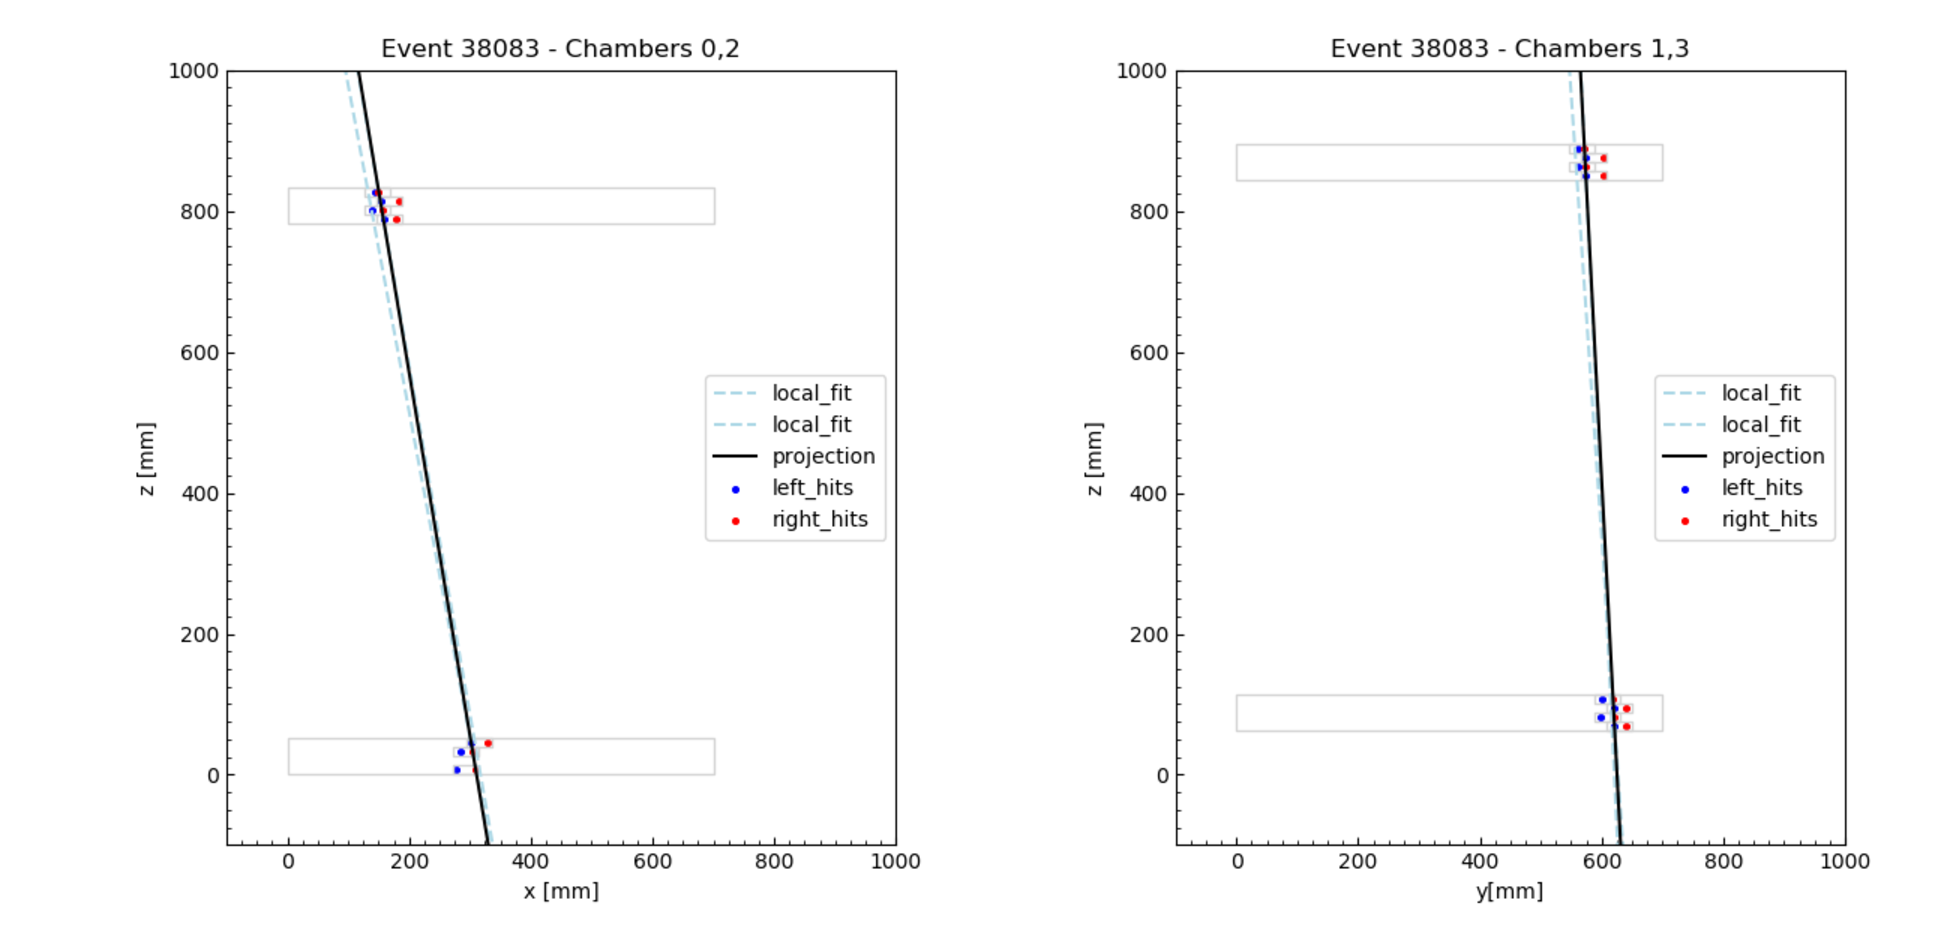
\includegraphics[scale=0.4]{pictures/example_track2D.pdf}
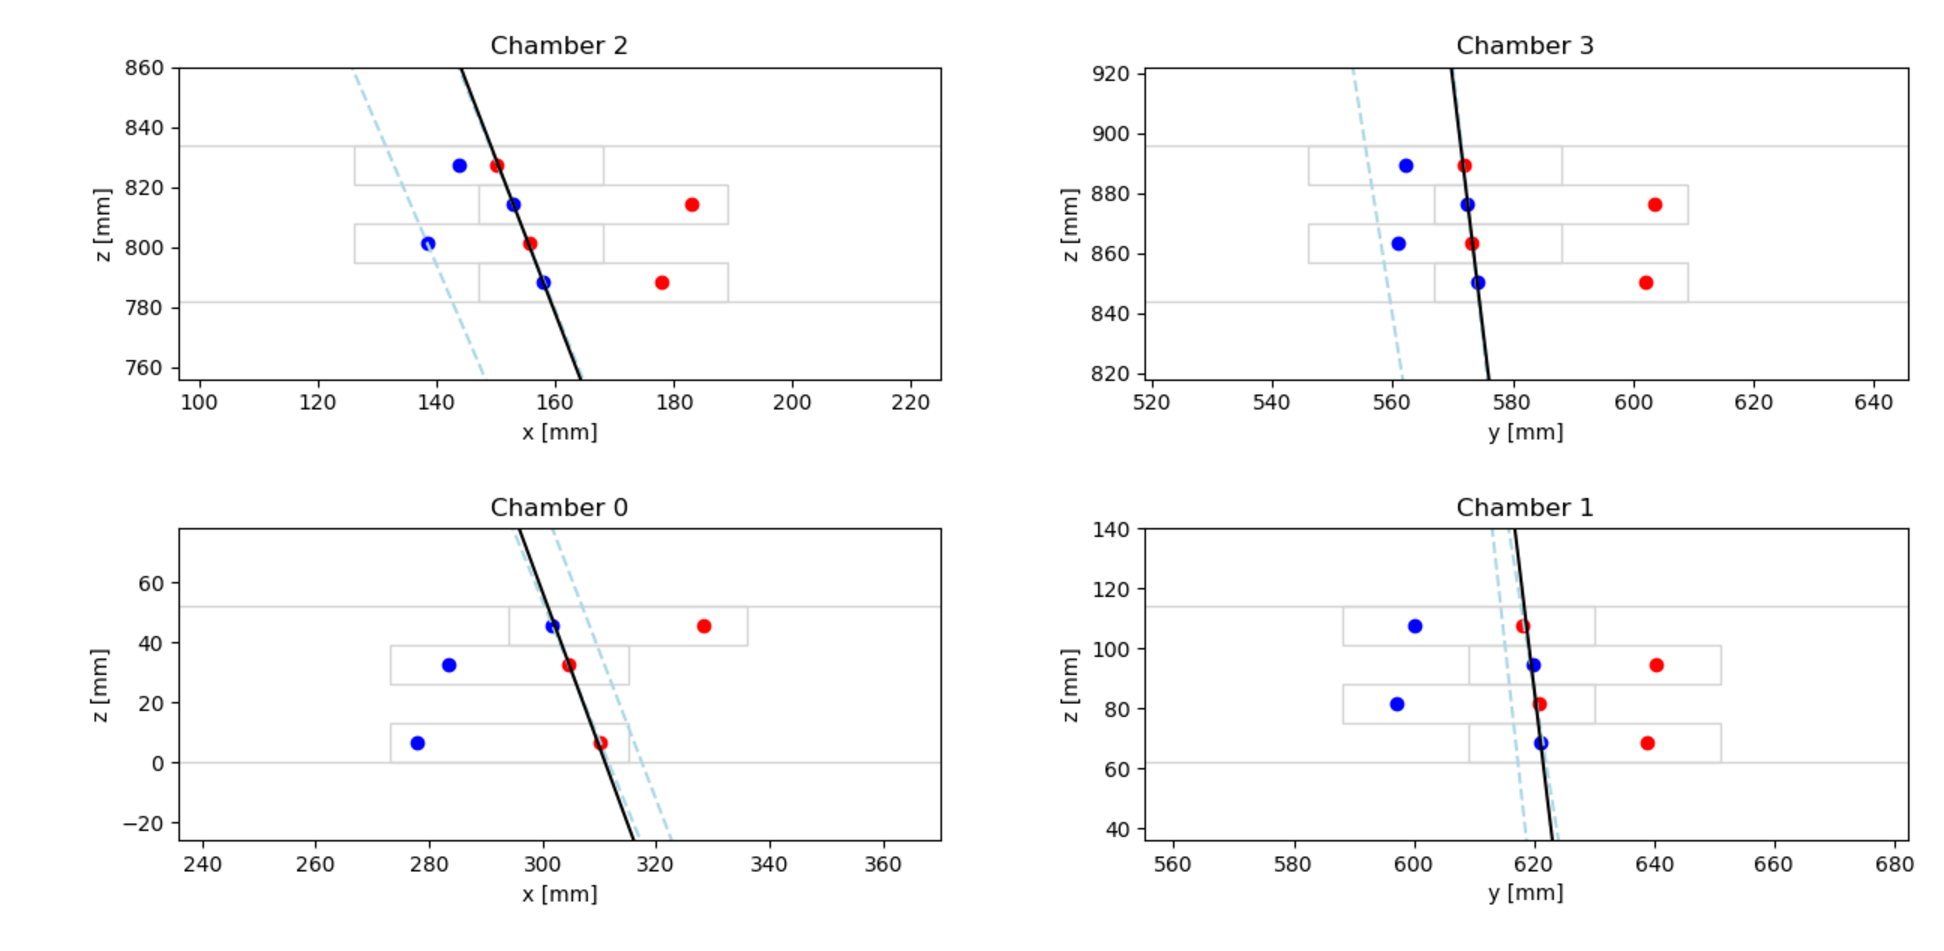
\includegraphics[scale=0.4]{pictures/example_track2D_dets.pdf}
\caption{Global and local projections of muon track}
\label{fig:glob_proj_ex}
\end{figure}


\section{Calibration}

Come tutti gli apparati strumentali, anche questo necessita di una fase di calibrazione.\\
A differenza di quando veniva usato come test beam, però, non è possibile raccogliere set di dati appositamente per queste operazioni, in quanto, con le camere rivolte verso l'alto sarebbe necessaria una fonte di muoni istallata sul tetto del laboratorio che invia continuamente segnali alle camere. Pertanto i dati stessi raccolti per l'analisi subiranno una fase di controllo preliminare necessaria alla stima dei parametri di calibrazione dell'apparato.\\
Sono due gli effetti principali che contribuiscono ad eventuali errori sistematici sulle posizioni dei punti: un'errata stima della velocità di deriva degli elettroni e una sovrastima/sottostima dei time pedestal. Attualmente il valore noto della velocità di deriva è:
\[ v_{drift} = XCELL/(2*T_{max}) = 42mm/(2*390ns) = 0.05385\hspace{1mm} mm/ns \]
mentre i time pedestal sono stati stimati con il metodo discusso in precedenza, e il loro effetto sulle misure è rappresentato in figura \ref{fig:DRIFT_TIMES}.\\
Per stimare i parametri di calibrazione, quindi, si procede analizzando i residui dei punti utilizzati per interpolare la traccia, definiti come la differenza tra il modulo della distanza filo-hit e il modulo della distanza tra il filo e il punto teorico (estrapolato dal fit). In particolare, se il t0 risulta sottostimato o sovrastimato questi residui dovranno essere in media minori o maggiori di zero, e lo si nota andando a computare degli opportuni istogrammi 1D per ogni camera (in quanto potrebbero necessitare di correzioni differenti). I risultati, riportati in figura \ref{fig:res1D} e in tabella \ref{tab:res1D} (nella quale sono rappresentati i parametri delle interpolazioni gaussiane ai singoli istogrammi), denotano che al momento non sono necessarie correzioni, in quanto i centroidi di tutte le distribuzioni sono compatibili con lo zero.

\begin{figure}[hbtp]
\begin{minipage}[c]{0.6\textwidth}
\centering
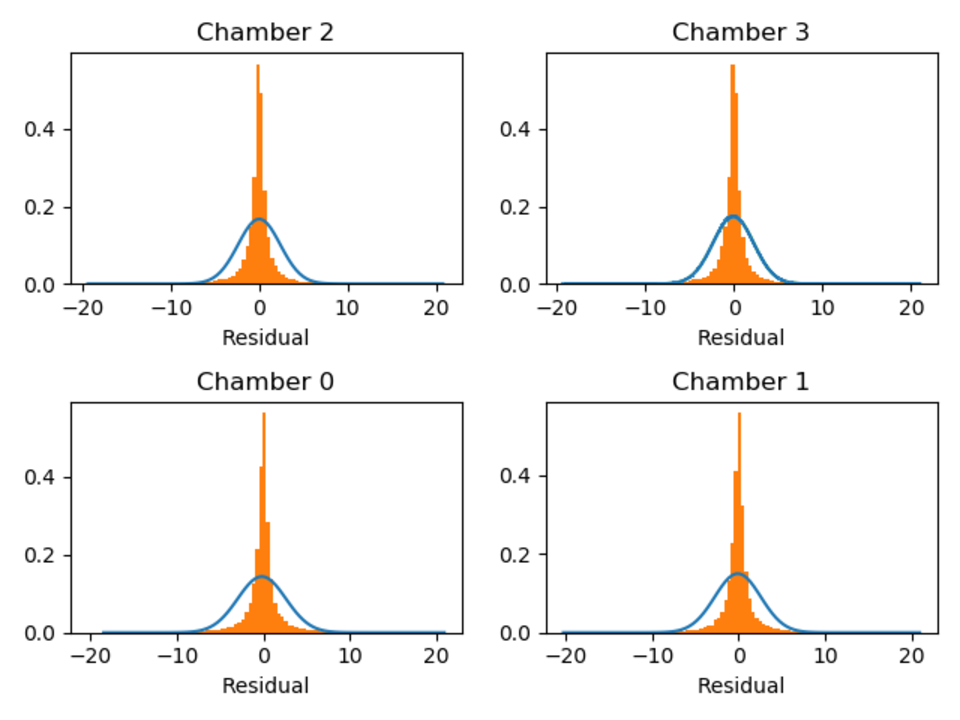
\includegraphics[scale=0.6]{pictures/Residuals_1D.pdf}
\caption{Residuals 1D of the four chambers}
\label{fig:res1D}
\end{minipage}\quad
\begin{minipage}[c]{0.4\textwidth}
\begin{tabular}{c | c  c}
\toprule
 \textbf{Chamber} & $\bm{\mu}$\textbf{ [mm]} & $\bm{\sigma}$\textbf{ [mm]}\\
0 & -0.17 & 2.8\\
1 & -0.11 & 2.7\\
2 & -0.02 & 2.38\\
3 &-0.09  & 2.29\\
\bottomrule
\end{tabular}
\caption{Parameters of the 1D residuals histograms}
\label{tab:res1D}
\end{minipage}
\end{figure}

\begin{figure}[hbtp]
\centering
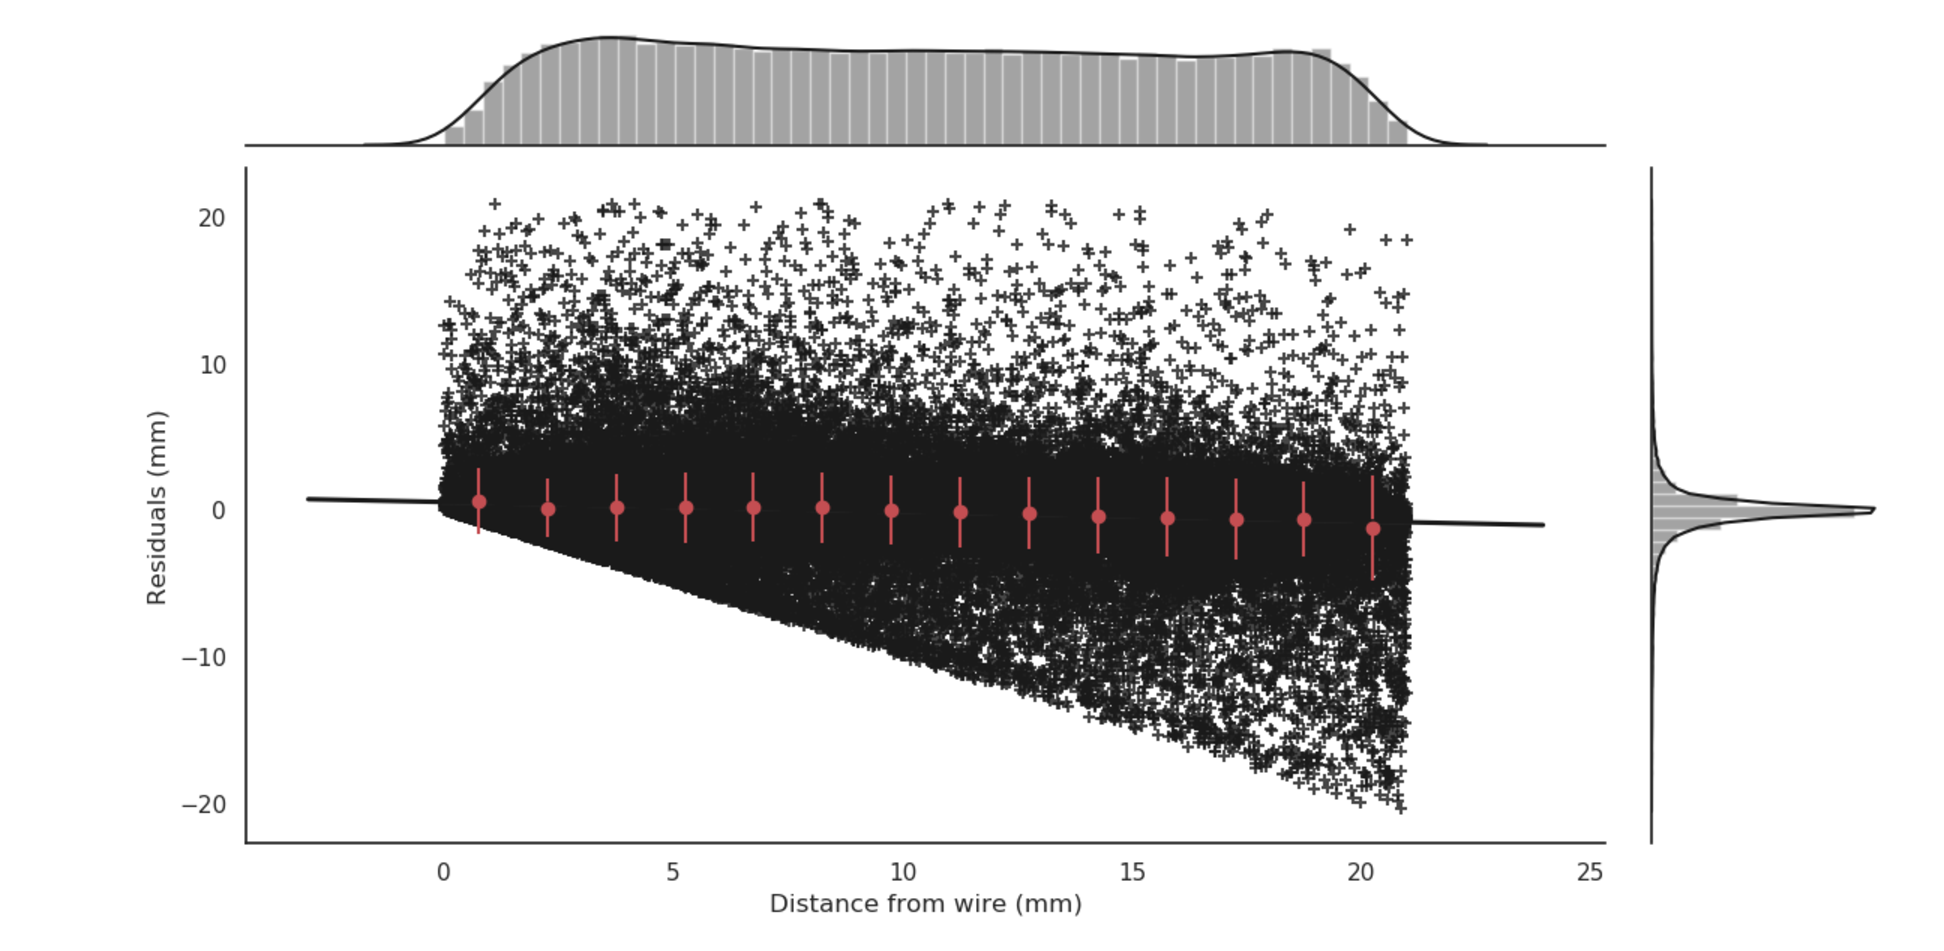
\includegraphics[scale=0.4]{pictures/Residuals_2D.pdf}
\caption{Residuals 2D}
\label{fig:res2D}
\end{figure}

Se invece fosse la velocità di deriva ad essere sbagliata, più ci si allontana dal filo, più i residui saranno mediamente diversi da zero. Questa analisi può essere effettuata andando alla ricerca di un trend nella distribuzione bidimensionale dei residui, riportata in figura \ref{fig:res2D}, nella quale i valori evidenziati rappresentano media ed errore dei punti in una piccola regione del grafico (e sono utili per stimarne al meglio l'andamento generale).\\ 
Per essere più precisi, nel grafico \ref{fig:res2D}, sono rappresentati i residui (definiti come $|x_{hit}-x_{wire}|-|x_{fit}-x_{wire}|$ in funzione della distanza dell'hit dal filo.\\

\begin{table}
\centering
\begin{tabular}{c  c}
\toprule
 \textbf{Slope} & \textbf{Intercept [mm]}\\
-0.066 & -0.584 \\
\bottomrule
\end{tabular}
\caption{Parameters of the linear interpolation}
\label{tab:res2D_analysis}
\end{table}


La tabella \ref{tab:res2D_analysis} riporta invece i parametri del fit lineare che si vede nel grafico. Dai numeri emersi si vede come il trend ricercato nella distribuzione non sia effettivamente presente (la pendenza è compatibile con 0), e pertanto, anche da questo punto di vista non è necessaria alcuna correzione dei punti.\\



\section{3D recostruction}

Una volta calcolate le proiezioni delle varie tracce (ed eventualmente corrette le posizioni dei punti se la calibrazione ha rivelato qualche incongruenza), si sfruttano relazioni puramente geometriche per ricostruire il passaggio del muone in tre dimensioni. In particolare si considerano i piani generati dalle due proiezioni e dalla direzione dei fili cui fanno riferimento (xz e asse y oppure yz e asse x) e ne si considera l'intersezione.\\
Il risultato (per l'evento a cui si è fatto riferimento prima) è il seguente:

\begin{figure}[hbtp]
\centering
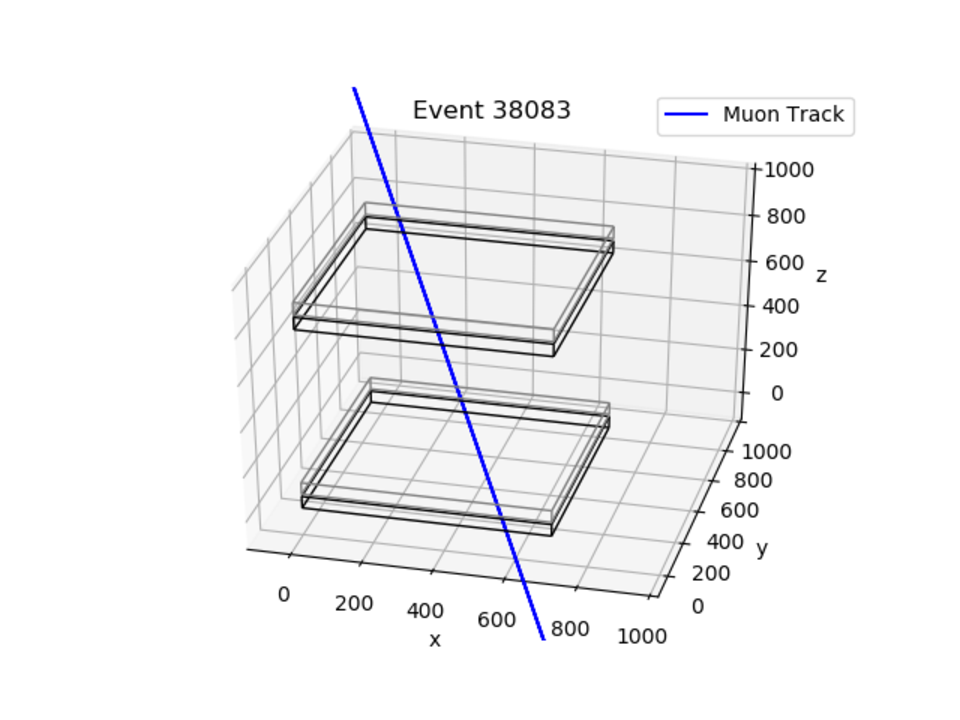
\includegraphics[scale=0.5]{pictures/Track_3D.pdf}
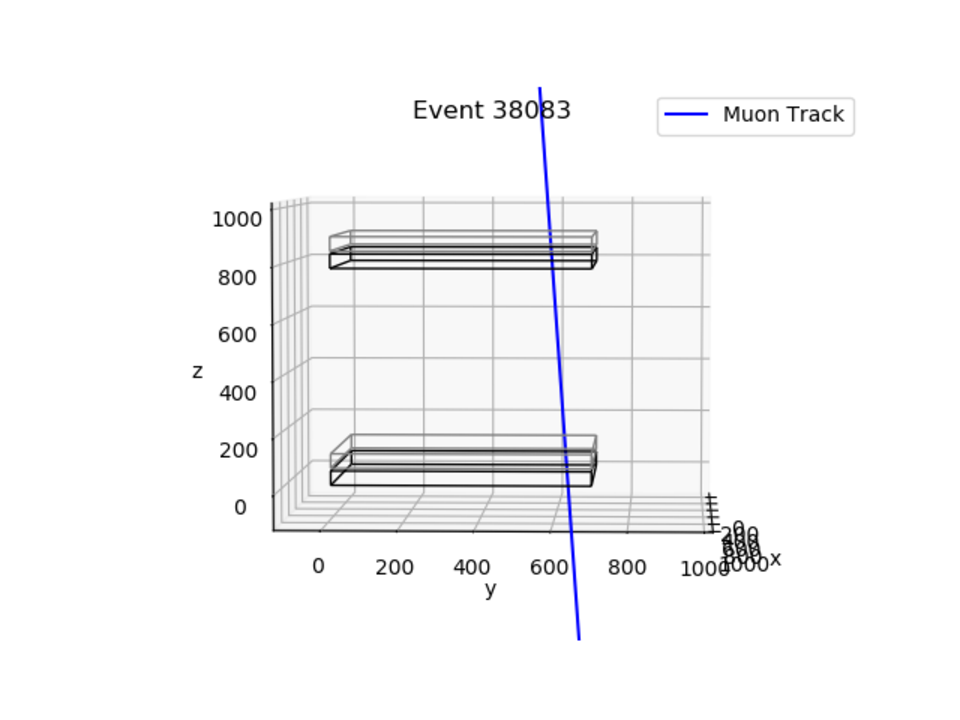
\includegraphics[scale=0.5]{pictures/Track_3D_2.pdf}
\caption{3D recostruction of muon track}
\label{fig:3D_track}
\end{figure}




\chapter{Analysis}

In questo capitolo si riportano invece alcune delle possibili analisi eseguibili a posteriori, una volta ricostruite tutte le tracce. In particolare ci si soffermerà sulla risoluzione angolare dell'apparato e sulla frequenza con cui vengono individuati eventi buoni.\\

\section{Angular resolution}

Un ulteriore utile studio che è possibile effettuare per testare i limiti dell'apparato è la sua risoluzione angolare. In pratica, note le pendenze delle rette globali interpolanti è possibile valutare le massime inclinazioni con cui le camere riescono a lavorare, e ricostruire l'intera traccia. Definito l'angolo che si va a rappresentare come quello tra la retta e la direzione verticale (in entrambe le sezioni xz e yz) si ottengono i seguenti risultati, in figura \ref{fig:angles} e in tabella \ref{tab:angles}. \\
\begin{figure}[hbtp]
\begin{minipage}[c]{0.6\textwidth}
\centering
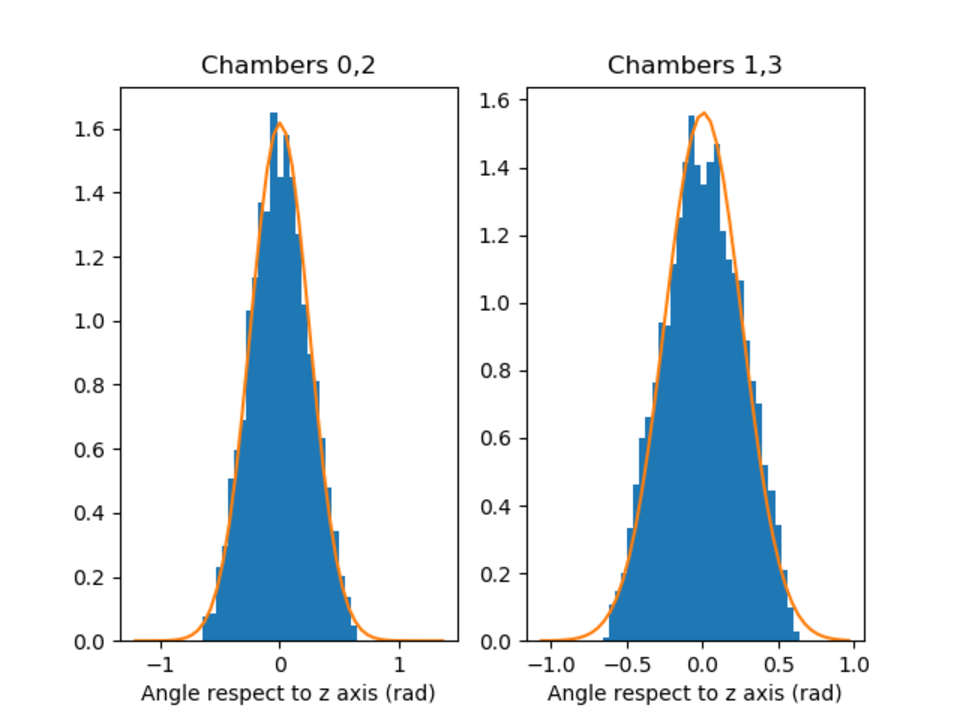
\includegraphics[scale=0.6]{pictures/Angles.pdf}
\caption{Graphical representation of angular resolution of the detectors}
\label{fig:angles}
\end{minipage} \quad
\begin{minipage}[c]{0.4\textwidth}
\begin{tabular}{c | c  c}
\toprule
 \textbf{Side} & $\bm{\mu}$\textbf{[rad]} & $\bm{\sigma}$\textbf{[rad]}\\
xz & 0.0037 & 0.25\\
yz & 0.0044 & 0.26\\
\bottomrule
\end{tabular}
\caption{Parameters of the interpolation}
\label{tab:angles}
\end{minipage}
\end{figure}

Una stima efficace della risoluzione angolare può quindi essere ottenuta calcolando la FWHM (= $2\sqrt{2\ln 2}\cdot\sigma$, ampiezze a mezza altezza) delle interpolazioni gaussiane appena effettuate. In tabella \ref{tab:angular_resolution} si riportano i risultati finali.\\

\begin{table}[hbtp]
\centering
\begin{tabular}{c c c}
\toprule
\textbf{Side} & \textbf{FWHM (rad)} & \textbf{Resolution (degrees)}\\
\midrule
xz & 0.59 & 33.80\\
yz & 0.61 & 34.95\\
\bottomrule
\end{tabular}
\caption{Angular resolution}
\label{tab:angular_resolution}
\end{table}

\section{Some statistics}

Qui di seguito (tabella \ref{tab:stats}), invece, si riportano informazioni utili, quali il numero di eventi ricostruiti nella prima parte del lavoro, rapportati a quelli che la seconda parte ha giudicato effettivamente "buoni".\\

\begin{table}[htbp]
\centering
\begin{tabular}{c|c}
\toprule
\textit{Total events analyzed} & 66541\\
\midrule
\textit{Good events selected} & 8080 (12.14 \%)\\
\bottomrule
\end{tabular}
\caption{Selection efficiency of the events}
\label{tab:stats}
\end{table}

La percentuale di good events è effettivamente piuttosto esigua, ma, come detto in precedenza, le richieste dell'algoritmo in questa seconda parte sono molto restrittive, nel senso che escludono con molta facilità gli eventi: basta che una delle camere sia anche solo troppo rumorosa rispetto alle altre per perdere tutto l'evento. Ma per quanto vincolante, la richiesta di avere tutti e 4 i detector "buoni" è necessaria per ricostruire tridimensionalmente la traccia. E inoltre quasi tutti gli eventi accettati sono come quello in figura \ref{fig:glob_proj_ex}, nel senso che sono segnali puliti, chiari e nei quali le diverse interpolazioni si sovrappongono quasi perfettamente. Inoltre non bisogna comunque trascurare la perdita di informazioni dovuta alle dead cell nel detector 0, le quali, in un metodo tanto delicato, possono risultare determinanti nello stabilire la bontà della camera.\\
Per quantificare il numero di eventi "quasi buoni", cioè scartati a causa di un errore presente in una sola delle camere, è sufficiente visionare la tabella \ref{tab:rejected_chamber}.\\

\begin{table}[htbp]
\centering
\begin{tabular}{c|c}
\toprule
\textit{Events rejected (only) by bad chamber 0} & 2322 (3.49\%) \\
\midrule
\textit{Events rejected (only) by bad chamber 1} & 717 (1.08\%) \\
\midrule
\textit{Events rejected (only) by bad chamber 2} & 281 (0.42\%) \\
\midrule
\textit{Events rejected (only) by bad chamber 3} & 1187 (1.78\%) \\
\bottomrule
\end{tabular}
\caption{Events rejected by one "bad" chamber}
\label{tab:rejected_chamber}
\end{table}

Come prevedibile, è proprio la camera 0 responsabile della reiezione di molti degli eventi.\\

Volendo, comunque, per guadagnare maggior statistica "bidimensionale", intesa come ristretta alle proiezioni sui piani xz e yz (ad esempio nel calcolo risoluzione angolare o nella stessa calibrazione) è sufficiente una lieve modifica al codice per cambiare la condizione di accettazione e richiedere che almeno una coppia di camere (e non più entrambe) mostrino una traccia globale.\\ 




\chapter{Conclusions}













\addcontentsline{toc}{chapter}{References}
\clearpage

\begin{thebibliography}{1}
\bibitem{nome del riferimento} Henley A. J., Wolf D., \textit{Learn Data Analysis with Python: Lessons in Coding}
\end{thebibliography}





\end{document}






